\documentclass[10pt,xcolor={usenames},fleqn,mathserif,serif]{beamer}

\hypersetup{pdfpagemode=FullScreen}

%% colors
\definecolor{bittersweet}{rgb}{1.0, 0.44, 0.37}
\definecolor{brilliantlavender}{rgb}{0.96, 0.73, 1.0}
\definecolor{antiquefuchsia}{rgb}{0.57, 0.36, 0.51}
\definecolor{violetw}{rgb}{0.93, 0.51, 0.93}
\definecolor{Veronica}{rgb}{0.63, 0.36, 0.94}
\definecolor{atomictangerine}{rgb}{1.0, 0.6, 0.4}
\definecolor{darkgray}{rgb}{0.66, 0.66, 0.66}
\definecolor{brightcerulean}{rgb}{0.11, 0.67, 0.84}
\definecolor{cadmiumorange}{rgb}{0.93, 0.53, 0.18}
\definecolor{ochre}{rgb}{0.8, 0.47, 0.13}
\definecolor{midnightblue}{rgb}{0.1, 0.1, 0.44}
\definecolor{lemon}{rgb}{1.0, 0.97, 0.0}
\definecolor{grey}{rgb}{0.7, 0.75, 0.71}
\definecolor{amber}{rgb}{1.0, 0.75, 0.0}
\definecolor{almond}{rgb}{0.94, 0.87, 0.8}
\definecolor{bf}{RGB}{88, 86, 88}
\definecolor{bb}{RGB}{177, 177, 177}
%%%%% Beamer SETUP
\usepackage{beamersetup}
%%%%%%%%%%%%%%%%%%%%%%%%%%%%%%%%%%% importa pacchetti
\usepackage{usepkg}
%%%%%%%%%%%%%%%%%%%%%%%%%%%%%%%%%%% Funzioni generali
\usepackage{functions}
%http://tex.stackexchange.com/questions/246/when-should-i-use-input-vs-include
\newcommand{\setmuskip}[2]{#1=#2\relax} %%problem usinig mu with calc (req by mathtools) loaded
%%% SOURCES
\usepackage{sources}


%\usepackage{length}
%%%%%%%%%%%%%%%%%%%%%%%%%%%%%%%%%%% Funzioni per questo file main
\usepackage{mathOp}

\def\status{coazione}%ripeter
\def\keeptrying{coazione}
\usepackage{LocalF}
%%%%%%%%%%%%%%%%%%%%%%%%%%%%%%%%%

\title{Sistemi planetari: formazione ed evoluzione (Beamer)}

% A subtitle is optional and this may be deleted
\subtitle{}

%\author{F.~Author\inst{1} \and S.~Another\inst{2}}
% - Give the names in the same order as the appear in the paper.
% - Use the \inst{?} command only if the authors have different
%   affiliation.

%\institute[Universities of Somewhere and Elsewhere] % (optional, but mostly needed)
%{
% \inst{1}
% Department of Computer Science\\
%  University of Somewhere
%  \and
%  \inst{2}%
%  Department of Theoretical Philosophy\\
%  University of Elsewhere}
% - Use the \inst command only if there are several affiliations.
% - Keep it simple, no one is interested in your street address.

\date{Febbraio, \today}
% - Either use conference name or its abbreviation.
% - Not really informative to the audience, more for people (including
%   yourself) who are reading the slides online

\subject{}
% This is only inserted into the PDF information catalog. Can be left
% out.

% Let's get started
\begin{document}

\begin{filecontents}{conservedvector.tex}

\centering
\begin{figure}
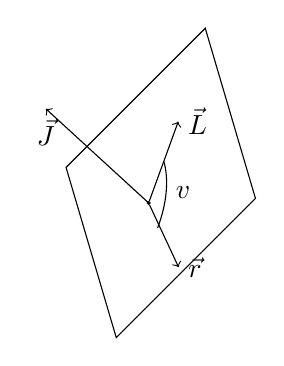
\begin{tikzpicture}[rotate around z=45, rotate around x=-45]
\draw (0,-0.3,0) -- (2.5,-0.3,0) -- (2.5,2.5,0) -- (0,2.5,0) -- cycle;
\draw[->] (1.,1.,0)node[draw,circle,inner sep=0] (o) {} -- (1.5,1.5,2)node[below] {$\vec{J}$};
\draw[->] (o) -- ++(295:0.9cm)node[right] {$\vec{r}$};
\draw[->] (o) -- ++(70:1.1cm)node[right] {$\vec{L}$}node [midway] (aux){};
\draw (aux) arc (0:-50:1) node[midway,right] {$v$};
\end{tikzpicture}

\label{fig:Lenztikz}

\end{figure}

\end{filecontents}


\begin{filecontents}{reducedproblem.tex}

%reduced problem

\begin{tikzpicture}

\node[circle,fill,inner sep=1pt,label=above:M] (M) at (0,0) {}; 
\draw (M)--++(30:1cm) node[circle,fill,inner sep=1pt,label=below:O] (O) {};
\draw[->] (O)--++(30:1.5cm) node[circle,fill,inner sep=1pt,label=above:m,yshift=1pt,xshift=1pt] (m) {} node[midway,above] {$\vec{r}$} ;

\node[circle,fill,inner sep=1pt,below=1cm of O,label=below:O] (O1) {}; 
\draw[->] (O1)--++(30:1.5cm) node[circle,fill,inner sep=1pt,label=above:m,yshift=1pt,xshift=1pt] (m1) {} node[midway,below] {$\vec{r_1}$} ;
\draw[->] (O1)--++(-150:1cm) node[circle,fill,inner sep=1pt,label=above:m,yshift=1pt,xshift=1pt] (m1) {} node[midway,below] {$\vec{r_2}$} ;
%\node (dida) at (7,0) {\parbox{8cm}{Siano m e M due masse puntiformi o a simmetria sferica: O \'e il centro di massa e $\vec{r}=\vec{r_1}-\vec{r_2}$ la distanza relativa.}};

\end{tikzpicture}

\end{filecontents}

\begin{filecontents}{ellipse.tex}

%ellisse

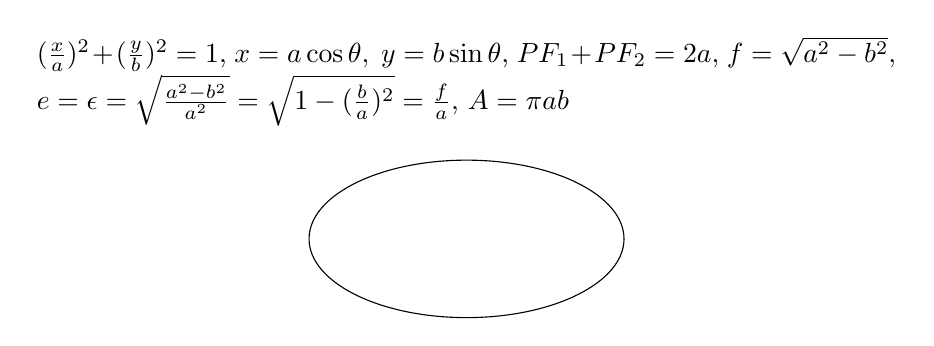
\begin{tikzpicture}

\draw ellipse (2cm and 1cm) node (o) {};
\node (prop) at (0,2) {\parbox{0.9\textwidth}{
$(\frac{x}{a})^2+(\frac{y}{b})^2=1$,
$x=a\cos{\theta},\ y=b\sin{\theta}$,
$PF_1+PF_2=2a$,
$f=\sqrt{a^2-b^2}$,
$e=\epsilon=\sqrt{\frac{a^2-b^2}{a^2}}=\sqrt{1-(\frac{b}{a})^2}=\frac{f}{a}$,
$A=\pi ab$}
};

\end{tikzpicture}

\end{filecontents}%%contain tikz files as filecontents

\addtobeamertemplate{block begin}{\setlength\abovedisplayskip{2pt}\setlength\belowdisplayskip{2pt}\setlength\abovedisplayshortskip{2pt}\setlength\belowdisplayshortskip{2pt}}

\addtobeamertemplate{block begin}{\vspace*{-3pt}}{}
\addtobeamertemplate{block end}{}{\vspace*{-3pt}}

\begin{frame}
  \titlepage
  Meta: wordonrame, errata, tolbf
\end{frame}

% Section and subsections will appear in the presentation overview
% and table of contents.
%\frame{\tableofcontents[onlyparts]}

\begin{frame}[allowframebreaks]{Sistemi planetari: formazione sistemi planetari, evoluzione dinamica e collisionale.}\phantomsection\linkdest{intro}
\tableofcontents[onlyparts]
\end{frame}

\begin{wordonframe}{To do}
\begin{itemize}
\item protstellar disk.
Simulation (bate18: diversity and statistical properties, larson 69,72, Tscharnuter 87,09)
Lifetime (richert 18: circumstellar disk lifetimes in numerous young stella rclusters)

\end{itemize}
\end{wordonframe}

\begin{wordonframe}{Perch\'e studio queste cose?? Sviluppi; futuro.}
\begin{columns}[T]\begin{column}{0.5\textwidth}
\begin{itemize}
\item Condizioni collasso nube molecolare e effetto di turbolenza rotazione e campi magnetici
\item Dischi protoplanetarii
\item schema a la Safronov e a la cameron
\item PPS: struttura disco gas/polvere, formazione planetesimi, accrescimento protopianeti, migrazione.
\item migrazione e instabilit\'a dinamiche
\end{itemize}
\end{column} \begin{column}{0.5\textwidth}
\begin{itemize}
\item Moto non kepleriano: perturbazioni.
\item Risonanze e regime caotico.
\item Effetti della radiazione
\item Evoluzione collisionale
\end{itemize}
\end{column}  \end{columns}

chaosorbit:
dynaevol: migrazione, stabilit\'a sistemi planetari,
physicaldescription: famiglie collisionali, anelli planetari, trasporto momento angolare
formationnizza: solar system formation neighborhood
saturnsystem: fisica degli anelli
\end{wordonframe}

\part{Formazione sistemi planetari}\linkdest{part:planetaryformation}
\section{Formazione stellare}\linkdest{cloudscollapse}

\subsection{Fase isoterma}

\begin{frame}{Collasso nube inter-stellare}
\begin{block}{Condizione di collasso}
Prima fase: collasso isotermo.
\begin{columns}
\begin{column}{0.5\textwidth}
$\TtwoDy{t}{I}<0$ quindi $E_T+U<0$.
\end{column}
\begin{column}{0.5\textwidth}
Nube di $H_2$ a $T=\SI{10}{\kelvin}$:
$\rho>\num{e-18}(\frac{M}{\msun{}})^{-2}$\si{\gram\per\cubic\cm}
\end{column}
\end{columns}
\begin{block}{Nubi giganti: addensamenti}
Turbolenza crea zone pi\'u dense: Mckee ostriker 07, Folin i 14, bertelli Motta 16.
\end{block}
\begin{block}{Rotazione}
\begin{columns}[T]
\begin{column}{0.5\textwidth}
T,M,J costanti:
\begin{align*}
&E_{th}\approx c'\\
&E_{Rot}\approx c''\rho\expy{\frac{2}{3}}\\
&U\approx c'''\rho\expy{\frac{1}{3}}\\
&\alpha=\frac{E_{th}}{U},\ \beta=\frac{E_{rot}}{U}
\end{align*}
\end{column}
\begin{column}{0.5\textwidth}
Condizione di collasso proibito: $16\alpha(\rho_0)\beta(\rho_0))>1$
\end{column}
\end{columns}
\end{block}
\end{block}
\end{frame}

\begin{wordonframe}{Collasso nube inter-stellare}\tolbf
\begin{block}{Teorema viriale:todo}\end{block}
\begin{columns}[T]
\begin{column}{0.5\textwidth}
T,M,J costanti:
\begin{align*}
&E_{th}\approx c'\\
&E_{Rot}\approx\frac{1}{2}\frac{J^2}{I}=\frac{J^2}{2}\frac{1}{\frac{2}{5}MR^2}=c''\rho\expy{\frac{2}{3}}\\
&U\approx\frac{3}{5}\frac{GM^2}{R}=c'''\rho\expy{\frac{1}{3}}
\end{align*}
\end{column}
\begin{column}{0.5\textwidth}
\begin{align*}
&f(\psi=\frac{\rho}{\rho_0})=\alpha_0\psi\expy{-\frac{1}{3}}+\beta_0\psi\expy{\frac{1}{3}}\\
&\begin{pmatrix}
&f<\frac{1}{2}: \text{collasso}\\
&f>\frac{1}{2}: \text{espansione}\\
\end{pmatrix}\\
&\alpha=\alpha_0(\rho_0)(\frac{\rho}{\rho_0})\expy{-\frac{1}{3}}\\
&\beta=\beta(\rho_0)(\frac{\rho}{\rho_0})\expy{\frac{1}{3}}
\end{align*}
\end{column}
\end{columns}
f ha minimo in $\psi_0=(\frac{\alpha_0}{\beta_0\beta_0})\expy{\frac{3}{2}}$
\end{wordonframe}

\subsection{Fase adiabatica}

\begin{frame}{Inizio fase adiabatica: aumento temperatura}
\begin{block}{Aumento cammino ottico}
\begin{columns}[T]
\begin{column}{0.5\textwidth}
Cammino ottico di un fotone minore delle dimensioni della nube: $\kappa\rho R>1$.
\end{column}
\begin{column}{0.5\textwidth}
Densit\'a che consente aumento T: $\rho_{ad}\propto M\expy{-\frac{1}{3}}?$
\end{column}
\end{columns}
\end{block}
\begin{block}{Termine collasso adiabatico ($\Delta E_T=-\Delta U$)}
Equilibrio: $E_T^{ad}+\Delta E_T=\frac{1}{2}|U+\Delta U|$: $\Delta R=-\frac{R}{2}$ e $\rho'=8\rho_{ad}$.
\end{block}
\begin{block}{Comportamento pseudo-adiabatico: $P\propto\rho\expy{\gamma}$}
\begin{columns}[T]
\begin{column}{0.5\textwidth}
\begin{align*}
&T=T_0(\frac{\rho}{\rho_{ad}})\expy{\gamma-1}\\
&P=P_0(\frac{\rho}{\rho_{ad}})\expy{\gamma}
\end{align*}
\end{column}
\begin{column}{0.5\textwidth}
$\gamma>\frac{4}{3}$: $\alpha$ diventa $>\frac{1}{2}$
\end{column}
\end{columns}
Condizione di equilibrio: $\rho_{eq}\propto M\expy{\theta}\begin{pmatrix}
\approx\num{e-10}, \gamma=\frac{5}{3}\\
\approx\num{e6}, \gamma=\frac{7}{5}
\end{pmatrix}$.
\end{block}
$T>\SI{e3}{\kelvin}$: dissociazione molecolare, ionizzazione.
Zona centrale raggiunge stato di quasi-equilibrio: lenta contrazione.
\end{frame}

\begin{wordonframe}{Fase adiabatica}
$P\propto\rho\expy{\gamma}$: corrisponde a vera adiabatica  se condizione iniziale di equilibrio o qe.

Condizione di equilibrio: $kT_0(\frac{\rho_{eq}}{\rho_{ad}})\expy{\gamma-1}=\const M\expy{\frac{2}{3}}\rho_{eq}\expy{\frac{1}{3}}$.

''Solo se la temperatura aumenta rapidamente con densit\'a \'e possibile ristabilire equilibrio.''

Ionizzazione e dissociazione rallentano aumento di T e P: accelerazione collasso.

Quando la zona interna raggiunge l'equilibrio l'esterno continua a contrarsi: rimbalzi.

\end{wordonframe}

\section{Formazione planetaria}\linkdest{protoplanetary}

\subsection{Osservazioni}

\begin{frame}{Cosa deve spiegare la teoria?}

\begin{itemize}
\item Massa nube interstellari molto maggiori della massa del sistema solare
\item stelle raggruppate in ammassi
\item Sistemi doppi o multipli
\item Numerosi sistemi planetari
\end{itemize}

\begin{itemize}
\item Frammentazione: presenza di condensazioni iniziali, fissione per rotazione. (moti turbolenti, jet di materia)
\item campi magnetici e rotazione inibiscono il collasso sul piano di simmetria
\item configurazioni simmetria cilindrica: toro, disco; rottura simmetria: spirale, strutture 3-assiali.
\item Popolazione Binarie strette ha picco popolazione per masse uguali, sistemi larghi hanno masse diverse (diversi canali formazione)
\item Problema momento angolare sistema solare. Trasferimento di momento verso l'esterno: turbolenza, magnetic breaking.
\end{itemize}

\end{frame}

\begin{wordonframe}{Cosa deve spiegare la teoria?}

Come si frammenta la nube interstellare? cosa differenzia l'evoluzione dei frammenti in sistemi doppi, sistemi planetari, etc

Problema momento angolare: $J_{\odot}/\msun{}=\SI{4e15}{\squared\cm\per\second}$, $J_{J}/M_J=\SI{4e20}{\squared\cm\per\second}$.

\end{wordonframe}

\begin{wordonframe}{Fatti osservativi di cui la teoria di formazione deve tenere conto}

\begin{itemize}
\item Orbite coplanari vicino all'equatore solare
\item Distanza tra orbite pianeti maggiore aumenta con distanza
\item Comete: Nube di Oort (\SI{e4}{\astronomicalunit}) con distribuzione isotropa, Kuiper belt ($>40\si{\astronomicalunit}$) con orbite planari.
\item 6 pianeti maggiori ruotano in maniera prograda con spin inclinato di meno di \ang{30}; Venere,Urano ruotano in maniera retrogada.
\item Sistemi di satelliti. Satelliti vicini al pianeta hanno piccola eccentricit\'a e inclinazione, viceversa quelli distanti.
\item I pianeti hanno $<0.2\%$ della massa del sistema solare.
\item $98\%$ del momento angolare \'e nel moto dei pianeti gioviani; il momento angolare dei satelliti dei pianeti gioviani \'e molto minore del momento dovuto allo spin dei pianeti.
\item Composizione: i pianeti terrestri sono pi\'u densi dei pianeti gioviani.
\item Fascia di asteroidi (origine meteoriti)
\item Crateri

\end{itemize}

\end{wordonframe}

\subsection{Modello nebulare}

\begin{frame}{Evoluzione disco di accrescimento}

Osservazione: $M_{d}\approx1-10^{-3}M_*$.

Tempo di vita del disco: la formazione di pianeti ha luogo quando il disco si \'e raffreddato a sufficienza.

Sistema solare: modelli a la Sofronov.

Sistemi extra-solari: modelli al la sofronov(/Cameron)

\end{frame}

\begin{wordonframe}{Accertion disk}

Dischi troppo massicci sono instabili

Inizialmente il disco riceve pi\'u massa dall'esterno di quanta cada sulla stella, successivamente perde massa fino ad esaurirsi.

La parte interna del disco si muove verso la stella, la parte esterna verso l'esterno; il confine tra le 2 zone si sposta verso l'esterno.

Problemi modello a la Cameron: dispersione maggior parte massa del disco, differenziazione composizione chimica pianeti giganti/Sole, mancanza di pianeti terrestri e corpi minori.

\end{wordonframe}

\section{Evoluzione del campo di velocit\'a di una nube interstellare: equazione di Eulero e Navier-Stokes.}

\begin{frame}{Evoluzione del campo di velocit\'a di una distro di materia.}


\begin{block}{Equazione di Eulero}
\begin{columns}[T]
\begin{column}{0.5\textwidth}
\begin{equation*}
\PDy{t}{\vec{v}}+(\scap{v}{\nabla})\cdot\vec{v}=-\frac{1}{\rho}\nabla P+\vec{g}
\end{equation*}
Non tiene conto di effetti dissipativi: viscosit\'a, scambi di calore.
\end{column}
\begin{column}{0.5\textwidth}
\begin{align*}
&\PDof{t}(v_i\rho)=-\PDof{x_k}\Pi_{ik}+\rho g_i\\
&\Pi_{ik}=P\delta_{ik}+\rho v_iv_k
\end{align*}
\end{column}

\end{columns}

\end{block}

\begin{columns}[T]

\begin{column}{0.45\textwidth}
\begin{block}{Tensore flusso d'impulso}
\begin{equation*}
\rho\PDy{t}{v_i}=-\rho v_k\PDy{x_k}{v_i}-\PDy{x_i}{P}+\rho g_i+\PDy{x_k}{\sigma_{ik}'}
\end{equation*}
\end{block}
\end{column}

\begin{column}{0.6\textwidth}
\begin{block}{Viscous stress tensor}
\begin{align*}
\sigma'_{ik}=\eta(\PDy{x_k}{v_i}+\PDy{x_i}{v_k}-\frac{2}{3}\delta_{ik}\PDy{x_l}{v_l})+\zeta\delta_{ik}\PDy{x_l}{v_l}
\end{align*}
\end{block}
\end{column}

\end{columns}

\begin{block}{Fluido incomprimibile: equazione di Navier-Stokes}
$\vec{g}=0$
\begin{equation*}
\rho\PDy{t}{\vec{v}}=-\rho(\scap{v}{\nabla})\vec{v}-\nabla P+\eta\nabla^2\vec{v}
\end{equation*}
\end{block}

\end{frame}

\begin{wordonframe}{Equazione del moto fluido: eq Eulero Navier-Stokes}

Descrizione euleriana: $\TDy{t}{\vec{v}}=\PDy{t}{\vec{v}}+\sum_i\PDy{x_i}{\vec{v}}\TDy{t}{x_i}=\PDy{t}{\vec{v}}+(\scap{v}{\nabla})\vec{v}$.

Flusso di momento:
\begin{equation*}
\PDof{t}(v_i\rho)=\rho\PDy{t}{v_i}-v_i\PDy{x_k}{(\rho v_k)}=-\PDof{x_k}(\rho v_iv_k)-\delta_{ik}\PDy{x_k}{P}+\rho g_i=-\PDof{x_k}\Pi_{ik}+\rho g_i
\end{equation*}

Viscous stress tensor: Nullo per moto uniforme; nullo per rotazione uniforme; composto da termini della forma $\PDy{x_k}{v_i}$.
$\zeta, \eta>0$: coefficienti di viscosit\'a, se variano lentamente con la posizione:
\begin{equation*}
\PDy{x_k}{\sigma'_{ik}}=\eta\PtwoDy{x_k}{v_i}+(\zeta+\eta/3)\PDof{x_i}\PDy{x_k}{v_k}
\end{equation*}

\end{wordonframe}

\section{Stabilit\'a: Criterio di jeans}\linkdest{stability}

\begin{frame}{Criterio di Jeans}

Mezzo infinito, non viscoso, in equilibrio $\vec{v}=0$, $P_0,\rho_0,\phi_0$ costanti nello spazio.

\begin{block}{Perturbazione isoterma}

\begin{columns}[T]
\begin{column}{0.5\textwidth}
\begin{align*}
&P_1=\frac{kT}{2m_p}\rho_1=c_s^2\rho_1\\
&\PDy{t}{\rho_1}+\rho_0\scap{\nabla}{v_1}\\
&\rho_0\PDy{t}{\vec{v}_1}=-\rho_0\nabla\phi_1-\nabla P_1\\
&\nabla^2\phi_1=4\pi G\rho_1
\end{align*}
\end{column}

\begin{column}{0.5\textwidth}
\begin{align*}
&\vec{v}_1=\vec{v}_{10}\exp{i(\scap{k}{x}-\omega t)}\\
&P_1=P_{10}\exp{i(\scap{k}{x}-\omega t)}\\
&\rho_1=\rho_{10}\exp{i(\scap{k}{x}-\omega t)}\\
&\phi_1=\phi_{10}\exp{i(\scap{k}{x}-\omega t)}
\end{align*}
\end{column}
\end{columns}
\end{block}

\begin{block}{Pi\'u piccola massa che pu\'o collassare}

\begin{equation*}
\omega^2=k^2c_s^2-4\pi G\rho_0
\end{equation*}

Per $\omega$ immaginaria si ha una soluzione che cresce esponenzialmente: perturbazioni instabili hanno
\begin{equation*}
k<k_J=\sqrt{4\pi G\rho_0\frac{2m_p}{kT}}\ \Rightarrow\ M_J=\frac{4}{3}\pi\rho_0(\frac{\lambda_J}{4})^3\propto T\expy{\frac{3}{2}}\rho_0\expy{-\frac{1}{2}}m_p\expy{-\frac{3}{2}}
\end{equation*}

\end{block}

\end{frame}

\begin{wordonframe}{Criterio di Jeans}
Non \'e soddisfatta eq. Poisson $\nabla^2\phi=4\pi G\rho$.
$M_J$ \'e la pi\'u piccola massa che pu\'o collassare; all'aumentare di $\rho$ $M_J$ diminuisce: fenomeni di frazionamento anche se \'e probabile coalescenza nella massa collassante complessiva.
Per $\omega\to 0$ (teorema del viriale):
\begin{align*}
&c_s^2=\frac{4\pi G\rho_0}{k^2}=4\pi\rho_0\lambda^2G\approx\frac{GM}{r}\\
&c_s^2\approx\frac{E}{m}\approx\frac{P}{\rho}
\end{align*}
\end{wordonframe}

\subsection{Effetto di turbolenza e campi magnetici}

\begin{frame}{Effetto della turbolenza e dei campi magnetici}

\begin{block}{Effetti di frenaggio}

\begin{columns}[T]
\begin{column}{0.5\textwidth}
\begin{align*}
&c_s^2\to c_s^2+v_{turb}^2\\
&k_J=\frac{\Omega_J}{\sqrt{c_s^2+v_{turb}^2}}\\
&M_J^{turb}\propto\rho\lambda_J^3\propto\frac{v_{turb}\expy{\frac{3}{2}}}{\sqrt{\rho}}
\end{align*}
\end{column}
\begin{column}{0.5\textwidth}
\begin{align*}
&P_G\to P_G+P_{mag}\\
&c_s^2\to c_s^2+\frac{B^2}{4\pi\rho_0}\\
&M_J^{mag}\propto\frac{B^3}{\rho^2}
\end{align*}

\end{column}
\end{columns}

\end{block}

\begin{block}{La turbolenza favorisce disomogeneit\'a di densit\'a}
\end{block}

\begin{block}{Campo magnetico in nubi ionizzate}

\begin{columns}[T]

\begin{column}{0.5\textwidth}
Campo magnetico congelato: $B\propto\rho\expy{\frac{2}{3}}$ quindi $M_J^{mag}=\const{}$.
\end{column}

\begin{column}{0.5\textwidth}
La diffusione ambipolare scongela il campo magnetico: $B\propto\rho^q,\ q<\frac{2}{3}$.
\end{column}

\end{columns}

\begin{block}{L'effeto del campo magnetico rompe la simmetria.}

\end{block}

\end{block}

\end{frame}

\begin{wordonframe}{Criterio di Jeans: effetto di campo magnetico e turbolenza}

$M_J^{turb,mag}$ indicano la massa di Jeans nei casi in cui la turbulenza/campi magnetici dominano su agitazione termica.

La turbolenza crea disomogeneit\'a che possono favorire il collasso.

Ionizzazione materia collassante aumenta conduzione: il campo magnetico \'e congelato. Il flusso del campo si conserva:
\begin{equation*}
\phi=Br^2\ \Rightarrow\ B\propto\rho\expy{\frac{2}{3}}
\end{equation*}

Per nubi molecolari giganti in presenza di campo magnetico galattico (\numrange{e-5}{e-6}G) l'effetto del campo magnetico \'e rilevante.

Il passaggio di materia in collasso pu\'o avvenire lungo/attraverso linee di forza del campo magnetico: non effetto di pressione ma rottura simmetria.


\end{wordonframe}


\subsection{Effetto della rotazione}

\begin{frame}{Criterio di Jeans: rotazione uniforme.}

\begin{block}{Il collasso sul piano ortogonale a $\vec{\Omega}$ \'e ostacolato}

\begin{align*}
&\delta v\approx\Omega\lambda\approx\frac{\Omega}{k}\Rightarrow c_s^2\to c_s^2+\frac{\Omega^2}{k^2}\\
&\omega^2=c_s^2k^2+\Omega^2-\Omega_J^2\\
&M_J\propto\frac{\rho c_s^3}{(4\pi G\rho-\Omega^2)\expy{\frac{3}{2}}}
\end{align*}

\end{block}

\begin{block}{Sfera uniforme}

\begin{equation*}
\beta=\frac{E_{rot}}{U}=(\frac{\Omega}{\Omega_J})^2
\end{equation*}

\end{block}

\begin{block}{Caso realistico}
\begin{equation*}
\Omega^2=\chi\beta\Omega_J^2:\ M_J(\beta)=\frac{M_J(0)}{(1-\chi\beta)\expy{\frac{3}{2}}}
\end{equation*}
\end{block}

\end{frame}

\begin{wordonframe}{Effetto rotazione uniforme sul criterio di jeans}

Energia gravitazionale di una sfera uniforme di raggio R e massa M: $U=-\frac{3}{5}\frac{GM^2}{R}$ e $E_{rot}=\frac{1}{5}MR^2\Omega^2$.

\end{wordonframe}

\begin{frame}{Criterio di Jeans: rotazione differenziale.}

\begin{block}{Relazione di dispersione in disco di accrescimento}
\begin{equation*}
\omega^2=c_s^2k^2-\Omega_J^2+\frac{2\Omega}{r}\PDof{r}(\Omega r^2)
\end{equation*}
\end{block}

\begin{block}{Rotazione differenziale dovuta al moto kepleriano}
\begin{align*}
&\Delta v\propto (\frac{1}{\sqrt{r}}-\frac{1}{\sqrt{r+\lambda}})\propto\lambda r\expy{-\frac{3}{2}}\approx\frac{\omega_{kep}}{k}\\
&\omega^2=c_s^2k^2-\Omega_J^2+\omega_{kep}^2
\end{align*}

\begin{columns}[T]

\begin{column}{0.5\textwidth}
Instabilit\'a per $4\pi G\rho>\frac{GM_*}{r^3}$.
\end{column}

\begin{column}{0.5\textwidth}
Formazione embrione planetario 
\begin{equation*}
\rho\geq(\frac{1.44\rsun{}}{a})^3\rho_{\odot}\approx\frac{\msun{}}{a^3}
\end{equation*}
\end{column}

\end{columns}

Per $a=a_J$: $\rho_{cr}\approx\SI{4e-9}{\gram\per\cubic\cm}$.

\end{block}

\end{frame}

\begin{wordonframe}{Effetto della rotazione.}

Frequenza epiciclica in disco di accrescimento: $\kappa=\frac{2\Omega}{r}\PDof{r}(\Omega r^2)$; considero moto kepleriano attorno a una stella $\Omega\approx\omega_{kep}$.

Limite di Roche approssimativo: $r>R_*(\frac{\rho_*}{3\rho})\expy{\frac{1}{3}}$. Condizione instabilit\'a: $M_{N}>\frac{M_*}{3}$.

Condizione formazione planetesimo:
\begin{align*}
&\frac{m_p}{M_*}\geq12(\frac{\delta}{r})^3\\
&\rho\geq\rho_{\odot}12(\frac{\rsun{}}{a})^3
\end{align*}

Limite di Roche: rottura di un satellite tenuto insieme da forze gravitazionali/ condizione necessaria perch\'e condensazioni autogravitanti possano svilupparsi.

\end{wordonframe}

\section{Instabilit\'a del disco di accrescimento}\linkdest{accretion}

\begin{frame}{Massa di Jeans in disco di accrescimento}
\begin{columns}[T]
\begin{column}{0.4\textwidth}
\begin{align*}
&\rho_{cr}>\num{e-18}(\frac{M}{\msun{}})\expy{-2}\si{\gram\per\cubic\cm}\\
&M_J\propto\rho\expy{-\frac{1}{2}}[\frac{T}{m_p}]\expy{\frac{3}{2}}
\end{align*}
\end{column}
\begin{column}{0.6\textwidth}
\begin{align*}
&M_{disk}\approx\frac{H}{a}\msun{}\\
&m_{pl}\approx (\frac{M_{disk}}{\msun{}})^3a^3\rho_{cr}\approx (\frac{M_{disk}}{\msun{}})^3\msun{}
\end{align*}
\end{column}
\end{columns}
Disco gassoso: condensazioni massicce.
\begin{block}{Modello a l\'a Safronov/Cameron}
\begin{columns}[T]
\begin{column}{0.5\textwidth}
\begin{equation*}
\rho(0)\approx(100q)\SI{e-10}{\gram\per\cubic\cm}
\end{equation*}
\end{column}
\begin{column}{0.5\textwidth}
$q\approx1$ (Cameron): condizioni critiche; $q\approx\num{e-2}$: $\rho(0)\ll\rho_{cr}$.
\end{column}
\end{columns}
Modelli a l\'a Safronov: $m_{dis}\approx\num{e-4}\msun{}$, $m_{pl}\approx\SI{e21}{\gram}$ ($\approx\SI{10}{\kilo\meter}$).
\end{block}
\begin{block}{Disco bidimensionale}
Disco freddo e sottile: tutte le particelle percorrono orbite kepleriane circolari; in un anello distante $r$ dalla stella e spesso $\delta r$, la condizione di condensazione \'e:
\begin{align*}
&\Delta E_{gra}\approx\frac{Gm_r^2}{r}>\Delta E\approx\frac{G\msun{}m_r}{r}(\frac{\delta r}{r})^2\\
&m_r<\frac{64\pi^2 r^4\exv{\rho}^2H^2}{\msun{}}\approx\frac{M_{dis}^2}{\msun{}}
\end{align*}
\end{block}
\end{frame}

\begin{wordonframe}{Modello Safronov/Cameron}
Zona di Giove, $T=100\si{\kelvin}$
\begin{align*}
&M_J\approx \msun{}: \rho>\SI{e-15}{\gram\per\cubic\cm}\\
&M_J\approx \num{e-3}\msun{}: \rho>\SI{e-9}{\gram\per\cubic\cm}
\end{align*}
Sedimentazione polvere in disco sottile: $M_J\to\num{e-18}M_J$: corpo solido (approx \SI{100}{\meter}).

\begin{block}{Modello disco 2d}
Conservazione di E,J:
\begin{align*}
&\frac{R_J}{R_E}\approx1+(\frac{\delta r}{4r})^2\\
&\Delta E\approx-\frac{G\msun{}m_r}{r}[(\frac{\delta r}{4r})^2_f-(\frac{\delta r}{4r})^2_i]
\end{align*}

Per disco di polvere: $m_r<\num{e-8}\msun{}\approx\SI{e25}{\gram}$.

Un anello sottile pu\'o essere instabile per perturbazioni azimutali: sotto-condensazioni circolari pari alla larghezza dell'anello $m_{pl}\approx m_r\frac{\delta r}{r}\approx\frac{m_r^2}{M_{dis}}$.

\end{block}

\end{wordonframe}

\subsection{Criterio di Toomre}

\begin{frame}{Criterio di Toomre (1964)}

\begin{block}{Instabilit\'a in disco sottile in moto kepleriano}

\begin{columns}

\begin{column}{0.5\textwidth}
\begin{equation*}
\omega^2=c_s^2k^2-2\pi\sigma G|k|+\kappa^2
\end{equation*}
\end{column}
\begin{column}{0.5\textwidth}
Pressione/rotazione stabilizzano lunghezze d'onda piccole/grandi.
\end{column}

\end{columns}

Instabilit\'a per: $Q=\frac{\kappa c_s}{\pi G\sigma}<1$ ($\sigma>\sigma_c=\frac{\kappa c_s}{\pi G}$).

\end{block}

\end{frame}

\begin{wordonframe}{Criterio di Toomre}
(Sistema a 2 componenti: Jog-Solomon 1984)

Nella condizione limite l'instabilit\'a riguarda una lunghezza d'onda, allontanandosi dalla condizione limite nelle regioni instabili si ha un range crescente di lunghezze d'onda.

\end{wordonframe}

\section{Disco primordiale e planetesimi: nschemi di formazione}\linkdest{formationschemes}

\subsection{Condizione di instabilit\'a}

\begin{frame}{Schema a l\'a Safronov/Cameron}
\begin{block}{Disco minimale}
Ogni pianeta si \'e formato in un anello del disco iniziale la cui massa \'e quella che ristabilisce la proporzione fra le abbondanze dei varii elementi solari (o galattiche): $M_{disk}(\SI{50}{\astronomicalunit})\approx0.04\msun{}$.
\end{block}
\begin{block}{Schema a l\'a Safronov}
Sedimentazione della componente polverosa in disco di pi\'u piccola massa. Instabilit\'a della polvere. $M_{disk}\approx\numrange{e-1}{e-2}\msun{}$.
Accrezione blocchi solidi ($\approx\SI{1}{\meter}$).
\end{block}
\begin{block}{Modello alla Cameron}
Instabilit\'a gravitazionale dell'intero disco. $M_{disk}\approx\msun{}$.
\end{block}
\end{frame}

\begin{wordonframe}{Schema Safronov/Cameron}
\begin{block}{Densit\'a superficiale}
\begin{align*}
&\sigma(r)\approx(\frac{r}{\SI{8e13}{cm}})\expy{-\frac{3}{2}}\si{\gram\per\cubic\cm}\\
&\int^{\SI{50}{\astronomicalunit}}\sigma(r)\,dr=0.04\msun{}
\end{align*}
\end{block}
Schema a l\'a Safronov: sedimentazione polvere verso il piano equatoriale.
Il criterio di Jeans non \'e applicabile: potenziale gravitazionale non \'e costante. (Forze mareali)
\end{wordonframe}

\begin{frame}{Struttura verticale del disco}
\begin{block}{Equilibrio idrostatico}
\begin{equation*}
\TDy{z}{P}=-\rho g_z=-\rho\frac{GM}{a^2}\frac{z}{a}\ \Rightarrow\ \rho(z)=\rho(0)\exp{-\frac{GMm}{a^3kT}z^2}
\end{equation*}
\end{block}
\begin{block}{Spessore effettivo}
\begin{columns}[T]
\begin{column}{0.5\textwidth}
\begin{align*}
&H=\frac{1}{\rho(0)}\int\rho(z)\,dz\\
&\frac{H}{a}\approx\sqrt{\frac{akT}{GMm}}
\end{align*}
\end{column}
\begin{column}{0.5\textwidth}
Per $a_J$, $T\approx\SI{100}{\kelvin}$, $H_2$: $\frac{H}{a}\approx0.1$.
Equipartizione energia gas/polvere:
\begin{equation*}
(\frac{H}{a})_{pol}=(\frac{H}{a})_{gas}\sqrt{\frac{m_{gas}}{m_{pol}}}
\end{equation*}
\end{column}
\end{columns}
\end{block}
\begin{block}{Equilibrio radiativo con la stella}
\begin{equation*}
T\propto a\expy{-\frac{1}{2}}\ \Rightarrow\ \frac{H}{a}\propto a \expy{\frac{1}{4}}\ (\propto a \expy{\frac{1}{8}})
\end{equation*}
\end{block}
\begin{columns}[T]
\begin{column}{0.4\textwidth}
\begin{block}{Instabilit\'a della polvere}
\begin{equation*}
\rho_{pol}^{cr}\approx\frac{\msun{}}{a^3}=\rho_{gas}X_{pol}\frac{H_{gas}}{H_{pol}}
\end{equation*}
\end{block}
\end{column}
\begin{column}{0.6\textwidth}
\begin{block}{Ruolo turbolenza}
\begin{itemize}
\item Impedisce sedimentazione disco di polvere
\item Crea addensamenti potentialmente instabili (Johansen 2007)
\end{itemize}
\end{block}
\end{column}
\end{columns}
\end{frame}

\begin{wordonframe}{Struttura verticale del disco}
Assumendo che $P=\frac{kT}{m}\rho$.
Equilibrio termico con la stella: $T^4R^2=\const{}$. Energy flux: $T_e^P=T_e^*\sqrt{\frac{R_*}{r_{*P}}}$.
$m_{pol}\approx\num{e12}m_{gas}$.
\end{wordonframe}

\subsection{Evoluzione collisionale proto-pianeti}

\begin{frame}{Accrescimento dei planetesimi: collisioni.}
\begin{itemize}
\item $r_{pl}<b<\frac{Gm_{pl}}{v_r^2}=b_0$: incontro ravvicinato ($|U_{max}|>E_{kin}^{\infty}$).
\item $b>(\frac{m_{pl}}{3\msun{}})\expy{\frac{1}{3}}a=d_{Hill}$: passaggio a grande distanza.
\item $b_0<b<d_{Hill}$: deflessioni di direzione e verso casuali.
\end{itemize}
\begin{block}{Scattering $b>r_{pl}$: variazione velocit\'a relativa}
\begin{equation*}
\delta v_r=\underbrace{\frac{Gm_{pl}}{b^2}}_{\exv{a}}\underbrace{\frac{2b}{v_r}}_{\exv{\tau_{int}}}=\frac{2Gm_{pl}}{bv_r}
\end{equation*}
\end{block}
\begin{equation*}
b_0<b<d_{Hill}:\quad [\TDy{t}{v_r^2}]_{enc}=\int_{r_{pl}}^d2\pi bv_r\frac{\sigma n}{m_{pl}v_r}(\frac{2Gm_{pl}}{bv_r})^2\,db
\end{equation*}
\begin{block}{Urti anelastici: impatti}
\begin{equation*}
[\TDy{t}{v_r^2}]_{imp}=\pi r_{pl}^2(\frac{\sigma n}{m_{pl}v_r})v_r(-v_r)
\end{equation*}
\end{block}
\end{frame}

\begin{wordonframe}{evoluzione collisionale pp}
Dato semiasse a e eccentricit\'a media e i corpi si incontrano se compresi in fascia di larghezza ae,$v_r\approx ena$.
Densit\'a numerica planetesimi: $\rho_{pl}\approx\frac{\sigma n}{m_{pl}v_r}$.
Variazione velocit\'a relativa media $\exv{\delta v_r}$ 
Diffusione nello spazio delle velocit\'a: aumento $\exv{e}\approx\exv{i}$ (random walk), a meno di risonanze.
\begin{itemize}
\item $r_{pl}<b<\frac{Gm_{pl}}{v_r^2}=b_0$: incontro ravvicinato ($|U_{max}|>E_{kin}^{\infty}$).
\item $b>(\frac{m_{pl}}{3\msun{}})\expy{\frac{1}{3}}a=d_{Hill}$: passaggio a grande distanza.
\item $b_0<b<d_{Hill}$: deflessioni di direzione e verso casuali, $\exv{\delta v_r}=0$,
\begin{equation*}
[\TDy{t}{v_r^2}]_{enc}=\int_{r_{pl}}^d2\pi bv_r\frac{\sigma n}{m_{pl}v_r}(\frac{2Gm_{pl}}{bv_r})^2\,db
\end{equation*}
\end{itemize}
Lobo di Hill: nel problema a 3 corpi \'e la regione in cui l'influenza del pianeta prevale su quella solare. Zona di Giove:
\begin{equation*}
\frac{\rho_{pl}}{3\rho_{\odot}}\approx\frac{1}{4}\ \Rightarrow\ d=(\frac{\rho_{pl}}{3\rho_{\odot}})\expy{\frac{1}{3}}r_{pl}\frac{a}{\rsun{}}\approx600r_{pl}
\end{equation*}
\end{wordonframe}

\begin{frame}{Evoluzione della velocit\'a relativa}
\begin{block}{Il sistema evolve verso stato stazionario}
\begin{align*}
&\TDy{t}{v_r}=[\TDy{t}{v_r}]_{enc}+_?[\TDy{t}{v_r}]_{imp}=\pi\frac{\sigma n}{m_{pl}}r_{pl}v_r[(\frac{v_e}{v_r})^4\ln{(\frac{d}{r_{pl}})}-1]\\
&\tau\approx\frac{m_{pl}}{\pi r_{pl}^2\sigma n}\approx\SI{e6}{\year}
\end{align*}
Il sistema evolve in tempo $\tau$ verso stato stazionario con $v_r\approx v_e$.
\end{block}
\begin{block}{Runaway growth}
Il pianeta pi\'u massiccio cresce pi\'u velocemente: contributo gravitazionale alla sezione d'urto
\begin{equation*}
\sigma_{imp}=\pi b_i\approx\pi r_{pl}^2(1+\frac{v_e^2}{v_{\infty}^2})
\end{equation*}
Il frammento pi\'u grosso determina la dinamica dell'intera zona: $v_r^2=\frac{Gm_1}{\theta r_1}$.
\end{block}

\end{frame}

\begin{wordonframe}{Evoluzione $v_r$}

$\tau$ piccolo rispetto tempi crescita embrioni planetari.

$\theta$ ($\approx1-100$) parametro di Safronov, $m_1$, $r_1$ massa e raggio del maggior embrione.

($\sigma_i\propto r_{pl}^4$ for small $v_{\infty}$.

\end{wordonframe}

\subsection{Formazione pianeti giganti e corpi minori}

\begin{frame}{Formazione di corpi minori: evoluzione collisionale a grande $v_r$}
\begin{block}{Collisioni ad alta velocit\'a relativa}
La velocit\'a relativa aumenta con la massa dell'embrione planetario: $v_r^2=\frac{Gm_1}{\theta r_1}$.

Aumentano $\exv{e}$ e $\exv{i}$: fascia di cattura pi\'u ampia.
\end{block}
\begin{block}{Espulsione di materia nelle fasi finali di accumulazione}
\begin{equation*}
v_{es}=(\sqrt{2}-1)\sqrt{\frac{G\msun{}}{a}}
\end{equation*}
Perturbazioni di orbite esterne possono determinare deflessione verso l'interno: main belt, late heavy bombardament.
\end{block}

\end{frame}

\begin{wordonframe}{formazione corpi minori}
$v_{es}$ orbita circolare: $\theta_{es}=\frac{1}{3-2\sqrt{2}}\sqrt{\frac{G\msun{}}{a}}$; $\theta_{es}\approx100$ per pianeti esterni in fase finale di formazione.

Espulsione di grande quantit\'a di materia nelle fasi finali di accumulazione
\end{wordonframe}

\begin{frame}{Cattura di gas}
\begin{itemize}
\item Massa embrione planetario
\item Temperatura locale
\item Rapidit\'a di formazione del proto-pianeta
\end{itemize}
Il modello a l\'a Safronov spiega la differenza di composizione dei pianeti.
\end{frame}

\begin{wordonframe}{Capacit\'a degli embrioni planetari di catturare gas}
Pi\'u il gas \'e freddo pi\'u \'e probabile la cattura.
\end{wordonframe}

\subsection{Leggi di scala nel modello a l\'a Safronov}

\begin{frame}{Legge di Titus-Bode (Armellini): pianeti, satelliti maggiori.}
\begin{equation*}
a(\si{\astronomicalunit})=B+C 2^n,\quad B\approx0.4,\ C\approx0.3
\end{equation*}
\begin{itemize}
\item Pianeti catturano tutto il materiale in una fascia attorno all'orbita.
\item Le zone di cattura sono continue e non si sovrappongono.
\end{itemize}
\begin{align*}
&\Delta a_{tot}\approx[\exv{e}+(\frac{m_{pl}}{\msun{}})^{\xi}]\approx\const{}a\\
&a_{n+1}=a_n+\frac{\Delta a_n}{2}+\frac{\Delta a_{n+1}}{2}\ \Rightarrow\ \frac{a_n}{a_{n+1}}=\const
\end{align*}
Le deviazioni dall'andamento medio favoriscono l'isolamento dei pianeti.
\end{frame}

\begin{wordonframe}{Formulazione alla armellini di TB.}
I semiassi dei pianeti (satelliti maggiori) costituiscono una serie geometrica approssimata.

Cattura geometrica, $\exv{e}$ eccentricit\'a media corpi piccoli: $\Delta a\approx\exv{e}a$.

Cattura gravitazionale: $\Delta a\approx(\frac{m_{pl}}{\msun{}})\expy{\xi}a$, $\xi\approx\frac{1}{3}$ (lobo di Hill), $\xi\approx\frac{1}{4}$ (Dole 1960).

Ipotesi semplificativa: $\Delta a_{tot}=\Delta a _{geo}+\Delta a_{gra}$.
\begin{align*}
&\Delta a_{tot}\approx[\exv{e}+(\frac{m_{pl}}{\msun{}})^{\xi}]\approx\const{}a\\
&a_{n+1}=a_n+\frac{\Delta a_n}{2}+\frac{\Delta a_{n+1}}{2}\ \Rightarrow\ \frac{a_n}{a_{n+1}}=\const
\end{align*}
Dove $\exv{e}$ varia lentamente con a, $m_{pl}$ non troppo grande, $\xi$ piccolo.

Tenendo conto delle risonanze (Wisdom 80/Lissauer 95): $\Delta a\approx(\frac{m_{pl}}{\msun{}})\expy{\frac{2}{7}}a$.
\end{wordonframe}

\begin{frame}{Scaling law}
Condensazione di tutto il materiale: $m_{pl}=2\pi a\sigma\Delta a$.

\begin{equation*}
\Delta a=(\frac{m_{pl}}{\msun})\expy{\gamma}a\ \Rightarrow\ m_{pl}\propto a\expy{\frac{2}{1-\gamma}}\sigma\expy{\frac{1}{1-\gamma}}\msun{}\expy{-\frac{\gamma}{1-\gamma}}
\end{equation*}

Dischi massicci producono meno pianeti ma pi\'u grossi:
\begin{equation*}
N_p=\frac{M_{disk}}{m_{pl}}\propto(\frac{M_{disk}}{\msun{}})\expy{-\frac{\gamma}{1-\gamma}}
\end{equation*}
$\gamma=\frac{2}{7}$, $\gamma=\frac{1}{4}$, $\gamma=\frac{1}{3}$ (Hill).

\end{frame}

\begin{wordonframe}{Scaling law}
\begin{equation*}
M_{disk}=a^2\sigma\ \Rightarrow\ m_{pl}\propto M_{disk}\expy{\frac{1}{1-\gamma}}M_*\expy{-\frac{\gamma}{1-\gamma}}=M_{disk}(\frac{M_{disk}}{M_*})\expy{\frac{\gamma}{1-\gamma}}
\end{equation*}
\end{wordonframe}

\section{Migrazione planetaria}\linkdest{migration}

\begin{frame}{Problemi nei modelli di formazione}
\begin{itemize}
\item Assenza di asteroidi oltre \SI{3.3}{\astronomicalunit}.
\item Scarsezza di oggetti nella regione di Kuiper interna a Plutone.
\item Nei sistemi extra-solari sono osservati pianeti pi\'u massicci di Giove a distanze minori (Effetti di selezione)
\end{itemize}
I dischi circumstellari tipicamente osservati hanno masse caratteristiche dei modelli a l\'a Safronov.
\end{frame}

\begin{frame}{Processi che determinano migrazione planetaria}

\begin{itemize}
\item Interazione pianeti in formazione disco (Goldreich, Tremaine 1980).
\item Scattering pianeta-corpi minori sopravvissuti alla fase di formazione.
\item Instabilit\'a dinamica causata da presenza di 2 pianeti massicci in orbite vicine (Jumping Jupiters): osservati in sistemi extra-solari.
\end{itemize}

\end{frame}

\begin{frame}{Interazione disco-pianeta}
\begin{block}{Risonanze}
\begin{itemize}
\item Corotazione: frequenza orbitale del disco e del pianeta coincidono
\item Risonanze di Lindblad: migrazione verso l'interno (tipo I)
\end{itemize}
\end{block}

\begin{block}{Rallentamento migrazione}
$\tau_{mig}\propto\frac{1}{m_{pl}}$: caduta troppo rapida sulla stella
\begin{itemize}
\item Azione efficace risonanze di Lindblad impedito da formazione gap attorno al pianeta massiccio
\item per pianeti massicci si ha svuotamento anello attorno orbita planetaria
\item turbolenza su larga scala
\item campo magnetico della stella
\item interazioni mareali/scambi di massa stella/pianeta
\end{itemize}
\end{block}
\end{frame}

\begin{wordonframe}{interazione disco-pianeta: risonanze}
Vedi interazione satellite-anelli.

Orbita eccentrica: corotazione con diverse parti del disco.

Le risonanze di Lindblad interne tendono a far migrare il pianeta verso l'esterno e viceversa. L'effetto della risonanza esterna prevale regolarmente.

Il momento angolare scambiato ad ogni risonanza \'e proporzionale a $m_{pl}^2$.

Disco massiccio e pianeta massiccio determinano migrazione veloce. Il modello spiega la scarsezza di brown dwarf. In $\tau\approx\SI{e5}{\year}$ un pianeta di qualche massa terrestre spiraleggia sulla stella.

Fascia vuota attorno all'orbita: diffusione non riesce a mantenere uniforme la densit\'a.
Turbolenza introduce termine stocastiuco nella migrazione.

\end{wordonframe}

\subsection{Jumping Jupiters}

\begin{frame}{Stabilit\'a dinamica}
\begin{block}{Stabilit\'a dinamica sistema a 3 corpi}
\begin{equation*}
\Delta=a_2-a_1>2\sqrt{3}R_{H12}\approx2.4a_1(\mu_1+\mu_2)\expy{\frac{1}{3}},\ \mu_i=\frac{\mu_i}{M_*}
\end{equation*}
Per Sole-Giove-Saturno: $a_S-a_J=\SI{4.2}{\astronomicalunit}>\SI{1.4}{\astronomicalunit}$.
\end{block}
\begin{block}{Stabilit\'a dinamica sistema a molti corpi}
Simulazioni numeriche (Marzari, Weidenschilling 2002): 3 pianeti con $m_i\approx m_J$, $a_i=a_{i-1}+kR_{Hi,i-1}$.

Il risultato pi\'u probabile \'e l'espulzione di un pianeta e l'immissione di un altro su orbita interna eccentrica: per i sistemi pi\'u stretti sono spiegati dalla migrazione.
\end{block}
\end{frame}

\begin{wordonframe}{Stabilit\'a dinamica orbite}
Lobo di Hill: $R_{H12}=(\frac{m_1+m_2}{M_*})\expy{\frac{1}{3}}\frac{a_1+a_2}{2}$.

Limite alla migrazione dalla conservazione dell'energia:
\begin{align*}
&E_i=-\frac{GM_*}{2}(\frac{m_1}{a_1}+\frac{m_2}{a_2}+\frac{m_3}{a_3})\approx\const{}\\
&E_f=-\frac{GM_*}{2}(\frac{m_3}{a_{3f}}+\frac{m_2}{a_{2f}})\approx-\frac{GM_*m_3}{2a_{3f}}\\
&\Rightarrow a_{3f}\approx\frac{1}{\frac{1}{a_1}+\frac{1}{a_2}+\frac{1}{a_3}}>\frac{a_1}{3}
\end{align*}
Sistemi con pianeti relativamente vicini e orbite eccentriche hanno spesso pianeta massiccio esterno.
\end{wordonframe}

\section{Modello di Nizza della formazione del sistema solare}\linkdest{nizza}

\begin{frame}{Modello di Nizza}

Scattering planetesimi causa la migrazione dei pianeti giganti.

\begin{block}{Regione formazione pianeti giganti}
\begin{itemize}
\item Giove \SI{5.45}{\astronomicalunit} (\SI{5.2}{\astronomicalunit})
\item Saturno \SI{8.5}{\astronomicalunit} (\SI{1}{\astronomicalunit})
\item Urano e Nettuno \SI{11}{\astronomicalunit} e \SI{17}{\astronomicalunit}
\end{itemize}
\end{block}
\begin{block}{Late heavy bombardament}
Quando Saturno attraversa la risonanza $2:1$ con Giove si ha una fase di intensa eccitazione dinamica: crateri lunari datano a \SI{3.8}{\giga\year} fa. (cattura troiani)
\end{block}
\end{frame}


\part{Evoluzione dei sistemi planetari: forze gravitazionali e non, collisioni.}\linkdest{part:evolution}
\section{Perturbazioni al moto Kepleriano}\linkdest{sec:nkperturb}

\subsection{Perturbazioni del moto dei pianeti maggiori del sistema solare}

\begin{frame}{Equazione del moto e condizioni iniziali. Sistema solare.}
\begin{columns}[T]
\begin{column}{0.5\textwidth}
\begin{equation*}
\ddvec{x}_i=\sum_{\mathclap{\substack{j=0\\j\neq i}}}\frac{Gm_j}{|\vec{x}_j-\vec{x}_i|^3}(\vec{x}_i-\vec{x}_j)+\vec{a}_i
\end{equation*}
\end{column}
\begin{column}{0.5\textwidth}
\begin{block}{Source other than 9 planets newtonian interaction ($\vec{a}_i$)}
Satellites: $(m_s/m_p)(r_s/r_p)^2$.
\end{block}
\end{column}
\end{columns}
\begin{itemize}
\item General relativity. $\frac{G\msun{}}{c^2r}=\num{e-9}(\SI{1}{\astronomicalunit}/r)$.
\item Asteroids: $\num{e-9}\msun{}$. Noise.
\item Galaxy. Galaxy's tidal acceleration (ratio to Sun): $\num{e-11}(r/\SI{40}{\astronomicalunit})^3$ (negligible).
\item Passing star: tidal acceleration $\num{e-4}(r/\SI{40}{\astronomicalunit})^3$. a of most planets are adiabatic-invariants.
\item Solar mass loss. $\TDy{t}{\msun{}}=\num{e-13}\msun{}\si{\per\year}$. Slow orbital expansion (preserve relative frequencies)
\end{itemize}
\end{frame}

\begin{wordonframe}{Solar system perturbation beside 9 planet attraction}
\begin{itemize}
\item Satellites: Satellites mass is lumped in parent planet neglecting solar attraction on quadrupole moment of planet-satellite system. Fractional error (relative to solar attraction) for Moon-Earth system \num{e-7}.
\item Galaxy's Tidal acceleration: $-4\pi G\rho z\hat{z}$, $\rho\approx0.15\msun{}\si{\cubic\parsec}$ local galactic density.
\item Passing star: nearest approach at \SI{e3}{\astronomicalunit}, lasts \SI{100}{\year}.
\end{itemize}
\end{wordonframe}

\subsection{Equazioni di Gauss}

\begin{frame}{Perturbazione elementi osculanti}
\begin{block}{Forza perturbante per unit\'a di massa: $(R,W,T)$.}\end{block}
\begin{columns}[T]
\begin{column}{0.2\textwidth}
\input{osculperturb}
\end{column}
\begin{column}{0.8\textwidth}
\begin{block}{Variazione semi-assi, eccentricit\'a e inclinazione pianeti.}
\begin{align*}
&\TDy{t}{a}=\frac{2a^2}{GM}\TDy{t}{E}=\frac{2}{n\sqrt{1-e^2}}[Re\sin{f}+T(1+e\cos{f})]\\
&\xrightarrow{e\to0}\frac{2T}{n}
\end{align*}
\end{block}
\end{column}\end{columns}
\begin{align*}
&\TDy{t}{e}=\frac{1-e^2}{2ea}\TDy{t}{a}-\frac{hTa(1-e^2)}{GMea(1+e\cos{f})}\xrightarrow{e\to0}\frac{R\sin{f}2T\cos{f}}{na}\\
&\TDy{t}{i}=W\frac{\sqrt{1-e^2}\cos{(f+\omega)}}{na(1+e\cos{f})}\xrightarrow{e\to0}W\frac{\cos{(f+\omega)}}{na}
\end{align*}
\begin{columns}  \begin{column}{0.55\textwidth}
\begin{block}{Relazioni inverse}
$\Delta v_{\theta}=\frac{n\Delta a}{2}$, $\Delta v_r=na\frac{(\Delta e-\Delta a/a\cos{f})}{\sin{f}}$
\end{block}
\end{column} \begin{column}{0.45\textwidth}
\begin{block}{Drag force}
$T<0$, a diminuisce, per legge di keplero energia cinetica aumenta.
\end{block}
\end{column}\end{columns}
\end{frame}

\begin{wordonframe}{Equazioni di Gauss: perturbazioni elementi orbitali}
\begin{align*}
&E=-\gamma\frac{1}{2a}=-Gm_1m_2\frac{1}{2a}=-(\frac{Gm_2}{h})^2\frac{m_1}{2}(1-e^2)=-\frac{Gm_2m_1}{2a},\ \eta=\sqrt{1-e^2}\\
&h=\sqrt{GMa(1-e^2)},f:\text{ J per unit\'a di massa e anomalia vera}
\end{align*}
\begin{block}{Variazione a e modulo di h}
\begin{align*}
&\TDy{t}{E}=Rv_r+Tv_t=[R(e\sin{f})+T(1+e\cos{f}))]\frac{Gm}{h}\\
&\TDy{t}{a}=\frac{2a^2}{Gm}\TDy{t}{E}=\frac{2}{n\eta}[T+e(T\cos{f}+R\sin{f})]\\
&\TDy{t}{h}=\PDy{a}{h}\TDy{t}{a}+\PDy{e}{h}\TDy{t}{e}=\frac{GM}{2h}[(1-e^2)\TDy{t}{a}-2ea\TDy{t}{e}]\\
\end{align*}
\end{block}
\begin{block}{Orientation of osculating plane determined by $\hat{h}$ or $(i,\Omega)$.}
$h\TDy{t}{\hat{h}}=W(\vec{r}\wedge\hat{h})$: $\hat{h}$ ruota con velocit\'a angolare $W/h\vec{r}$. Split torque into component along line of node and perpendicular to it on orbit plane: $\TDy{t}{\Omega}=\frac{rW\sin{\omega+f}}{h\sin{i}}$,
$\TDy{t}{i}=\frac{rW\cos{\omega+f}}{h}$.
\end{block}
\end{wordonframe}

\subsection{Lagrange perturbation equations}

\begin{frame}{Lagrange perturbed equations}

\begin{block}{Lagrange's parenthesys of constant of motion is constant.}
\begin{align*}
&[F,G]=-[G,F]=\PDy{F}{q^i}\PDy{G}{p_i}-\PDy{G}{q^i}\PDy{F}{p^i}\\
&\{c_a,c_b\}[c_b,c_d]=-\delta_{ad}
\end{align*}
\end{block}
\begin{block}{Perturbing function}
Perturbing force conservative: $\vec{F}=-\nabla \phi_p$: $\TDy{t}{c_a}=\{c_a,\phi_p\}=\{c_a,c_b\}\PDy{c_b}{\phi_p}$. $H=H_0+\phi_p=\frac{1}{2}p^2-\frac{Gm}{r}+\phi_p$.
\end{block}
\end{frame}

\begin{wordonframe}{Lagrange perturbation equation}
\begin{equation*}
\phi_p(a,e,i,\Omega,\bar{\omega}=\omega+\Omega,\epsilon=\bar{\omega}+\epsilon';t), \epsilon'=nt-nt_0-\chi(t)\ \chi=\int ndt'
\end{equation*}
\begin{block}{orbital element (memo)}
\begin{columns}  \begin{column}{0.5\textwidth}
\begin{figure}[!ht]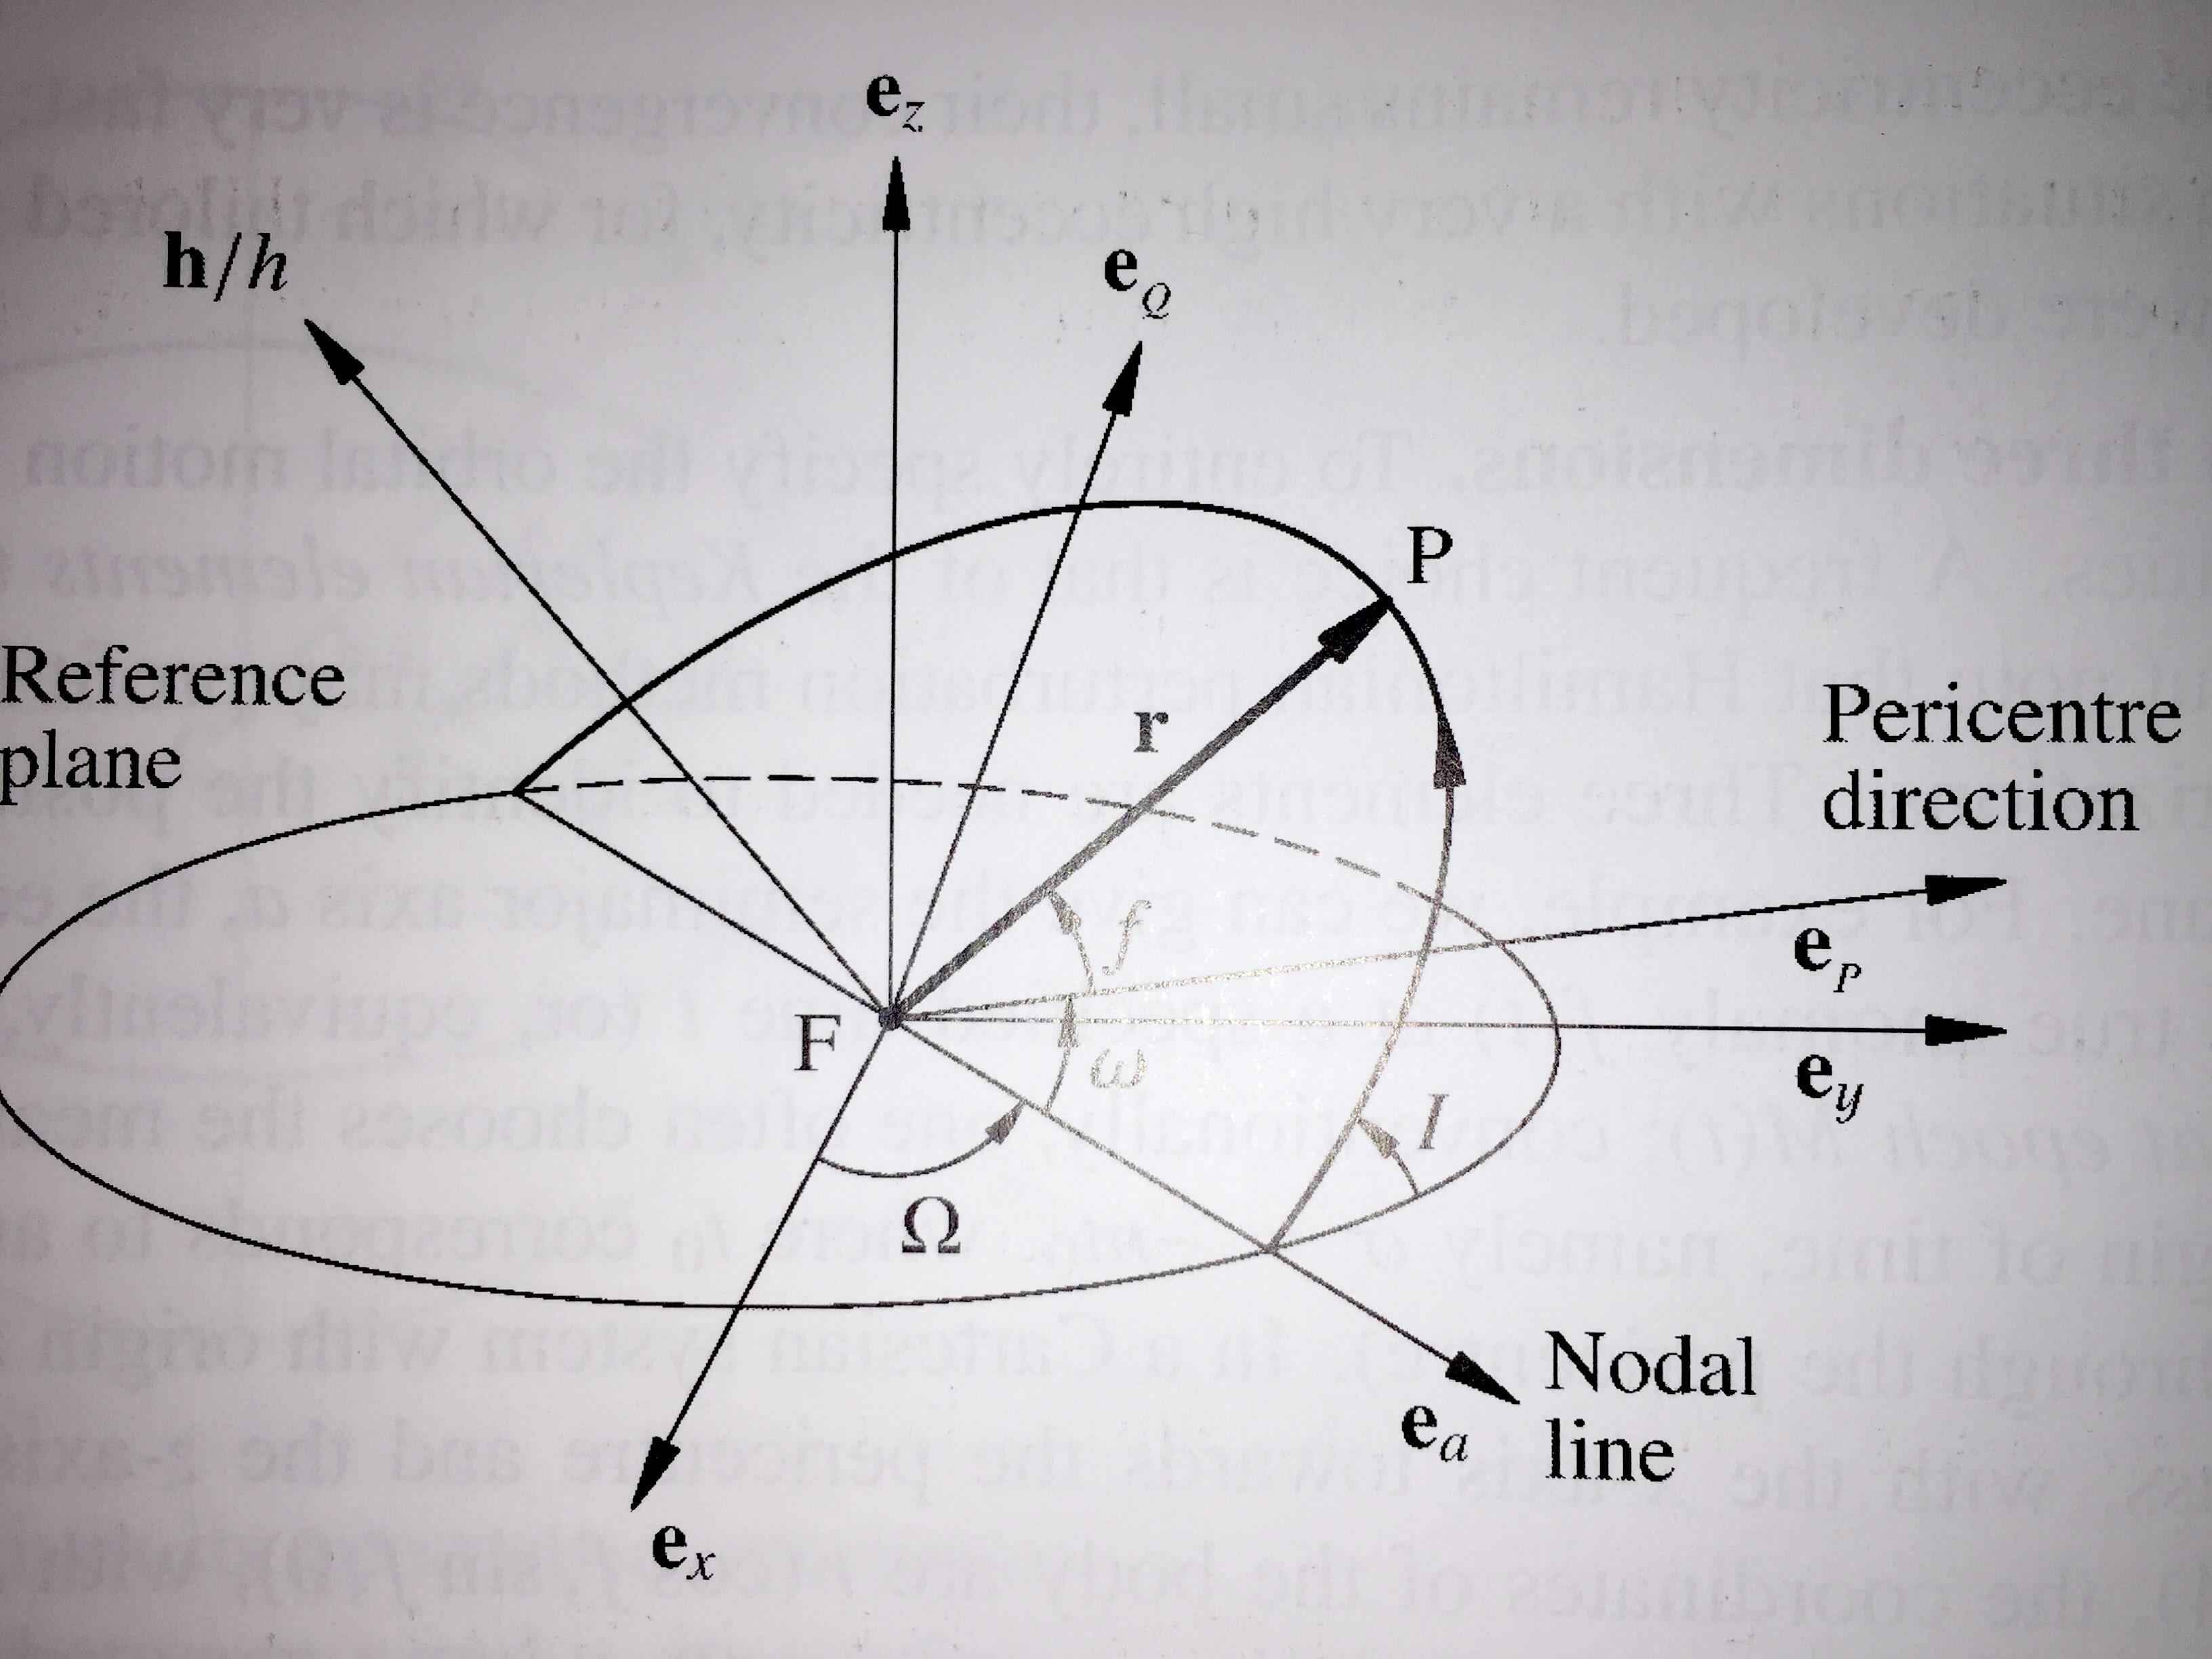
\includegraphics[width=0.95\textwidth]{orbitalbook}\end{figure}
\end{column} \begin{column}{0.5\textwidth}
\begin{align*}
&\hat{e}_P=\begin{pmatrix}\cos{\Omega}\cos{\omega}-\cos{I}\sin{\Omega}\sin{\omega}\\\sin{\omega}\cos{\Omega}+\cos{i}\cos{\Omega}\sin{\omega}\\\sin{i}\sin{\omega}\end{pmatrix}\\
&\hat{e}_Q=\hat{h}\wedge\hat{e}_P\\
&=\begin{pmatrix}-\cos{\Omega}\cos{\omega}-\cos{I}\sin{\Omega}\cos{\omega}\\-\sin{\omega}\sin{\Omega}+\cos{i}\cos{\Omega}\cos{\omega}\\\sin{i}\cos{\omega}\end{pmatrix}
\end{align*}
\end{column}  \end{columns}
\end{block}
\begin{columns}[T]\begin{column}{0.5\textwidth}
\begin{block}{Costanti del moto}
2N costanti del moto $c_a (N=3)$
\begin{align*}
\{H_0,c_a\}=0
\end{align*}
\end{block}
\end{column}\begin{column}{0.5\textwidth}
\begin{block}{Calcolo LP al pericentro)}
\begin{align*}
&\vec{r}=r[\cos{f}\hat{e}_P+\sin{f}\hat{e}_Q]\\
&\vec{v}=\frac{na}{\eta}[-\sin{f}\hat{e}_P+(e+\cos{f})\hat{e}_Q]
\end{align*}
\end{block}
\end{column}\end{columns}
\end{wordonframe}

\begin{frame}{Lagrange equation for perturbing function $\phi_p$}
\begin{align*}
&\frac{1}{a}\TDy{t}{a}=-\frac{2}{na^2}\PDy{\epsilon}{\phi_p}\\
&\TDy{t}{e}=\frac{\eta}{na^2e}[\PDy{\bar{\omega}}{\phi_p}+(1-\eta)\PDy{\epsilon}{\phi_p}]\\
&\TDy{t}{I}=\frac{1}{na^2\eta\sin{i}}[\PDy{\Omega}{\phi_p}+2\sin{i/2}(\PDy{\bar{\omega}}{\phi_p}+\PDy{\epsilon}{\phi_p})]\\
&\TDy{t}{\Omega}=-\frac{1}{na^2\eta\sin{i}}\PDy{i}{\phi_p}\\
&\TDy{t}{\bar{\omega}}=-\frac{\eta}{na^2e}\PDy{e}{\phi_p}-\frac{\tan{i/2}}{na^2\eta}\PDy{i}{\phi_p}\\
&\TDy{t}{\epsilon}=\frac{2}{na}\Dcvar{\PDy{a}{\phi_p}}{n}-\frac{\eta(1-\eta)}{na^2e}\PDy{e}        {\phi_p}-\frac{\tan{i/2}}{na^2\eta}\PDy{i}{\phi_p})
\end{align*}
%\begin{figure}[!ht]\includegraphics[height=0.45\textheight]{Lpertelem}\end{figure}
\end{frame}

\begin{frame}{Perturbazioni secolari}
\begin{columns}\begin{column}{0.5\textwidth}
\begin{block}{Perturbing function for 1 by 2}
\end{block}
\end{column}
\begin{column}{0.5\textwidth}
\begin{block}{periodic in angular variables $(\Omega_1,\bar{\omega}_1, \lambda_1; \Omega_2,\bar{\omega}_2, \lambda_2)$}\end{block}
\end{column}  \end{columns}
\begin{align*}
\phi_p=-Gm_2(\frac{1}{r_{12}}-\frac{\vec{r}_1\cdot\vec{r}_2}{r_2^3})\qquad\to\qquad \sum C_{ijk}\cos{\Phi_{ijk}}
\end{align*}
\begin{block}{Rate of change of elements of j-planets due to i}
\begin{align*}
&\mu=\frac{\phi_p}{Gm/a}=\frac{\phi_p}{n^2a^2}>=\frac{a_p}{n^2a}\\
&\TtwoDy{t}{\chi}\approx O(\mu n^2),\ \TDy{t}{c_i}(\frac{\dot{a}}{a}\approx O(\mu n)
\end{align*}
$a$ are stable to $\mu^2$ (Lagrange/Tisserand):no secular term over $\frac{1}{\mu^2}$ orbital period.
\end{block}
\begin{block}{mean orbital elements}
\begin{align*}
&(\TDy{t}{\vec{c}'_j})_i=\mu\exv{F_{ji}}=\frac{\mu}{(2\pi)^2}\iint^{2\pi}\,d\lambda_i\,d\lambda_j\mu F_{ji}(\vec{c}'_j,\lambda_j,\vec{c}'_i,\lambda_i)
\end{align*}
\end{block}
\end{frame}

\begin{wordonframe}{Perturbazioni elementi orbitali}
$\Dcvar{\TDy{t}{\vec{c}_a}}{i}=f_a(c_b(t),t)$, orbital phase $\TtwoDy{t}{\chi}$
\begin{align*}
&\vec{c}_i=(a_i,e_i,i_i,\bar{\omega}_i,\Omega_i,\epsilon_i)\\
&\lambda_i\text{: mean longitude}\leftrightarrow \chi=\int\,dt’\chi
\end{align*}
Perturbation function for planet 1
\begin{align*}
&\TtwoDy{t}{\vec{r}}=-G(\msun{}+m_1)\frac{\vec{r}_1}{r_1^3}+Gm_2(\frac{\vec{r}_2-vec{r}_1}{r_{12}^3}-\frac{\vec{r}_2}{r_2^3})\\
&=-\PDof{\vec{r}_1}[-\frac{G(\msun{}+m_1)}{r_1}+\phi_p]\\
&\phi_p=\sum C_{ijk}\cos{(i_1\lambda_1+i_2\lambda_2+j_1\bar{\omega}_1+j_2\bar{\omega}_2+k_1\Omega_1+k_2\Omega_2)}
\end{align*}
\end{wordonframe}

\section{Secular theory.}\linkdest{sec:secular}

\begin{frame}{Secular planetary theory ($\phi_p$ linearized in e,i)}
\begin{columns}[T]\begin{column}{0.5\textwidth}
\begin{block}{Non-singular elements}
\begin{align*}
&h=e\sin{\bar{\omega}},\ k=e\cos{\bar{\omega}}\\
&P=\sin{i}\sin{\Omega},\ Q=\sin{i}\cos{\Omega}
\end{align*}
\end{block}
\end{column}\begin{column}{0.5\textwidth}
\begin{block}{L perturbation equation linear in e,i (Long-term evolution)}
\begin{align*}
&\TDy{t}{h}=-\frac{1}{na^2}\PDy{k}{\phi_p},\ \TDy{t}{k}=\frac{1}{na^2}\PDy{h}{\phi_p}\\
&\TDy{t}{P}=-\frac{1}{na^2}\PDy{Q}{\phi_p},\ \TDy{t}{Q}=-\frac{1}{na^2}\PDy{P}{\phi_p}
\end{align*}
\end{block}
\end{column}\end{columns}
\begin{block}{Lagrange (linear) solution}
\begin{columns}[T]\begin{column}{0.5\textwidth}
\begin{align*}
&h_i=\sum_jR_{ij}\sin{(g_jt+\beta_j)},\\
&k_i=\sum_jR_{ij}\cos{(g_jt+\beta_j)}\\
&P_i=\sum_jS_{ij}\sin{(s_jt+\gamma_j)},\\
&Q_i=\sum_jS_{ij}\cos{(s_jt+\gamma_j)}
\end{align*}
\end{column}
\begin{column}{0.5\textwidth}
\begin{block}{ND harmonic oscillator}
\begin{align*}
&\TtwoDy{t}{\vec{h}'}=-B'^2\cdot\vec{h}',\ldots
\end{align*}
\end{block}
$g_j, s_j\approx O(\mu n)$ typ. period \SI{50}{\kilo\year}-few \si{\mega\year}, i,j from 1-N but labels modes not planets.
\begin{align*}
\sum_jm_jn_ja_j^2(h_j^2+k_j^2)=\sum_jm_jn_ja_j^2e_j^2=\const{}
\end{align*}
\end{column}\end{columns}
\end{block}
\end{frame}

\begin{wordonframe}{Secular planetary theory}
In solar system e,i are small $\approx \sqrt{\mu}$; $\vec{e}_i\cdot\vec{e}_j=h_ih_j+k_ik_j$.
\begin{align*}
&W_{ij}=m_j\exv{R_{ij}}=-[B_{ij}(h_ih_j+k_ik_j)+\frac{1}{2}B_{ii}(h_i^2+h_j^2+k_i^2+k_j^2)\\
&+C_{ij}(P_iP_j+Q_iQ_j)+\frac{1}{2}C_{ii}(P_i^2+P_j^2+Q_i^2+Q_j^2)]\\
&m_i,\vec{h}=h_i,\ldots\\
&h_i'=\sqrt{m_in_ia_i^2}h_i,\ k_i'=\sqrt{m_in_ia_i^2}k_i,\ B_{ij}'=B_{ij}/\sqrt{(m_jn_ja_j^2)(m_in_ia_i^2)}
\end{align*}
Lagranage equation in Hamiltonian form:
\begin{equation*}
\TDy{t}{\vec{h}'}=B'\cdot\vec{k}'\quad\TDy{t}{\vec{k}'}=-B'\cdot\vec{k}'
\end{equation*}
\begin{block}{secular resonances}
\begin{columns}[T]\begin{column}{0.6\textwidth}
located in surface in $(a,e,i)$ space: $g-g_i=0$ ($\nu_i$), $s-s_j=0$ ($\nu_{1j}$). When the forced contribution prevails values of some elements of a test body are determined by whole planetary dynamics. $g=B_{00}/(mna^2)$
\end{column}\begin{column}{0.4\textwidth}
\begin{figure}[!ht]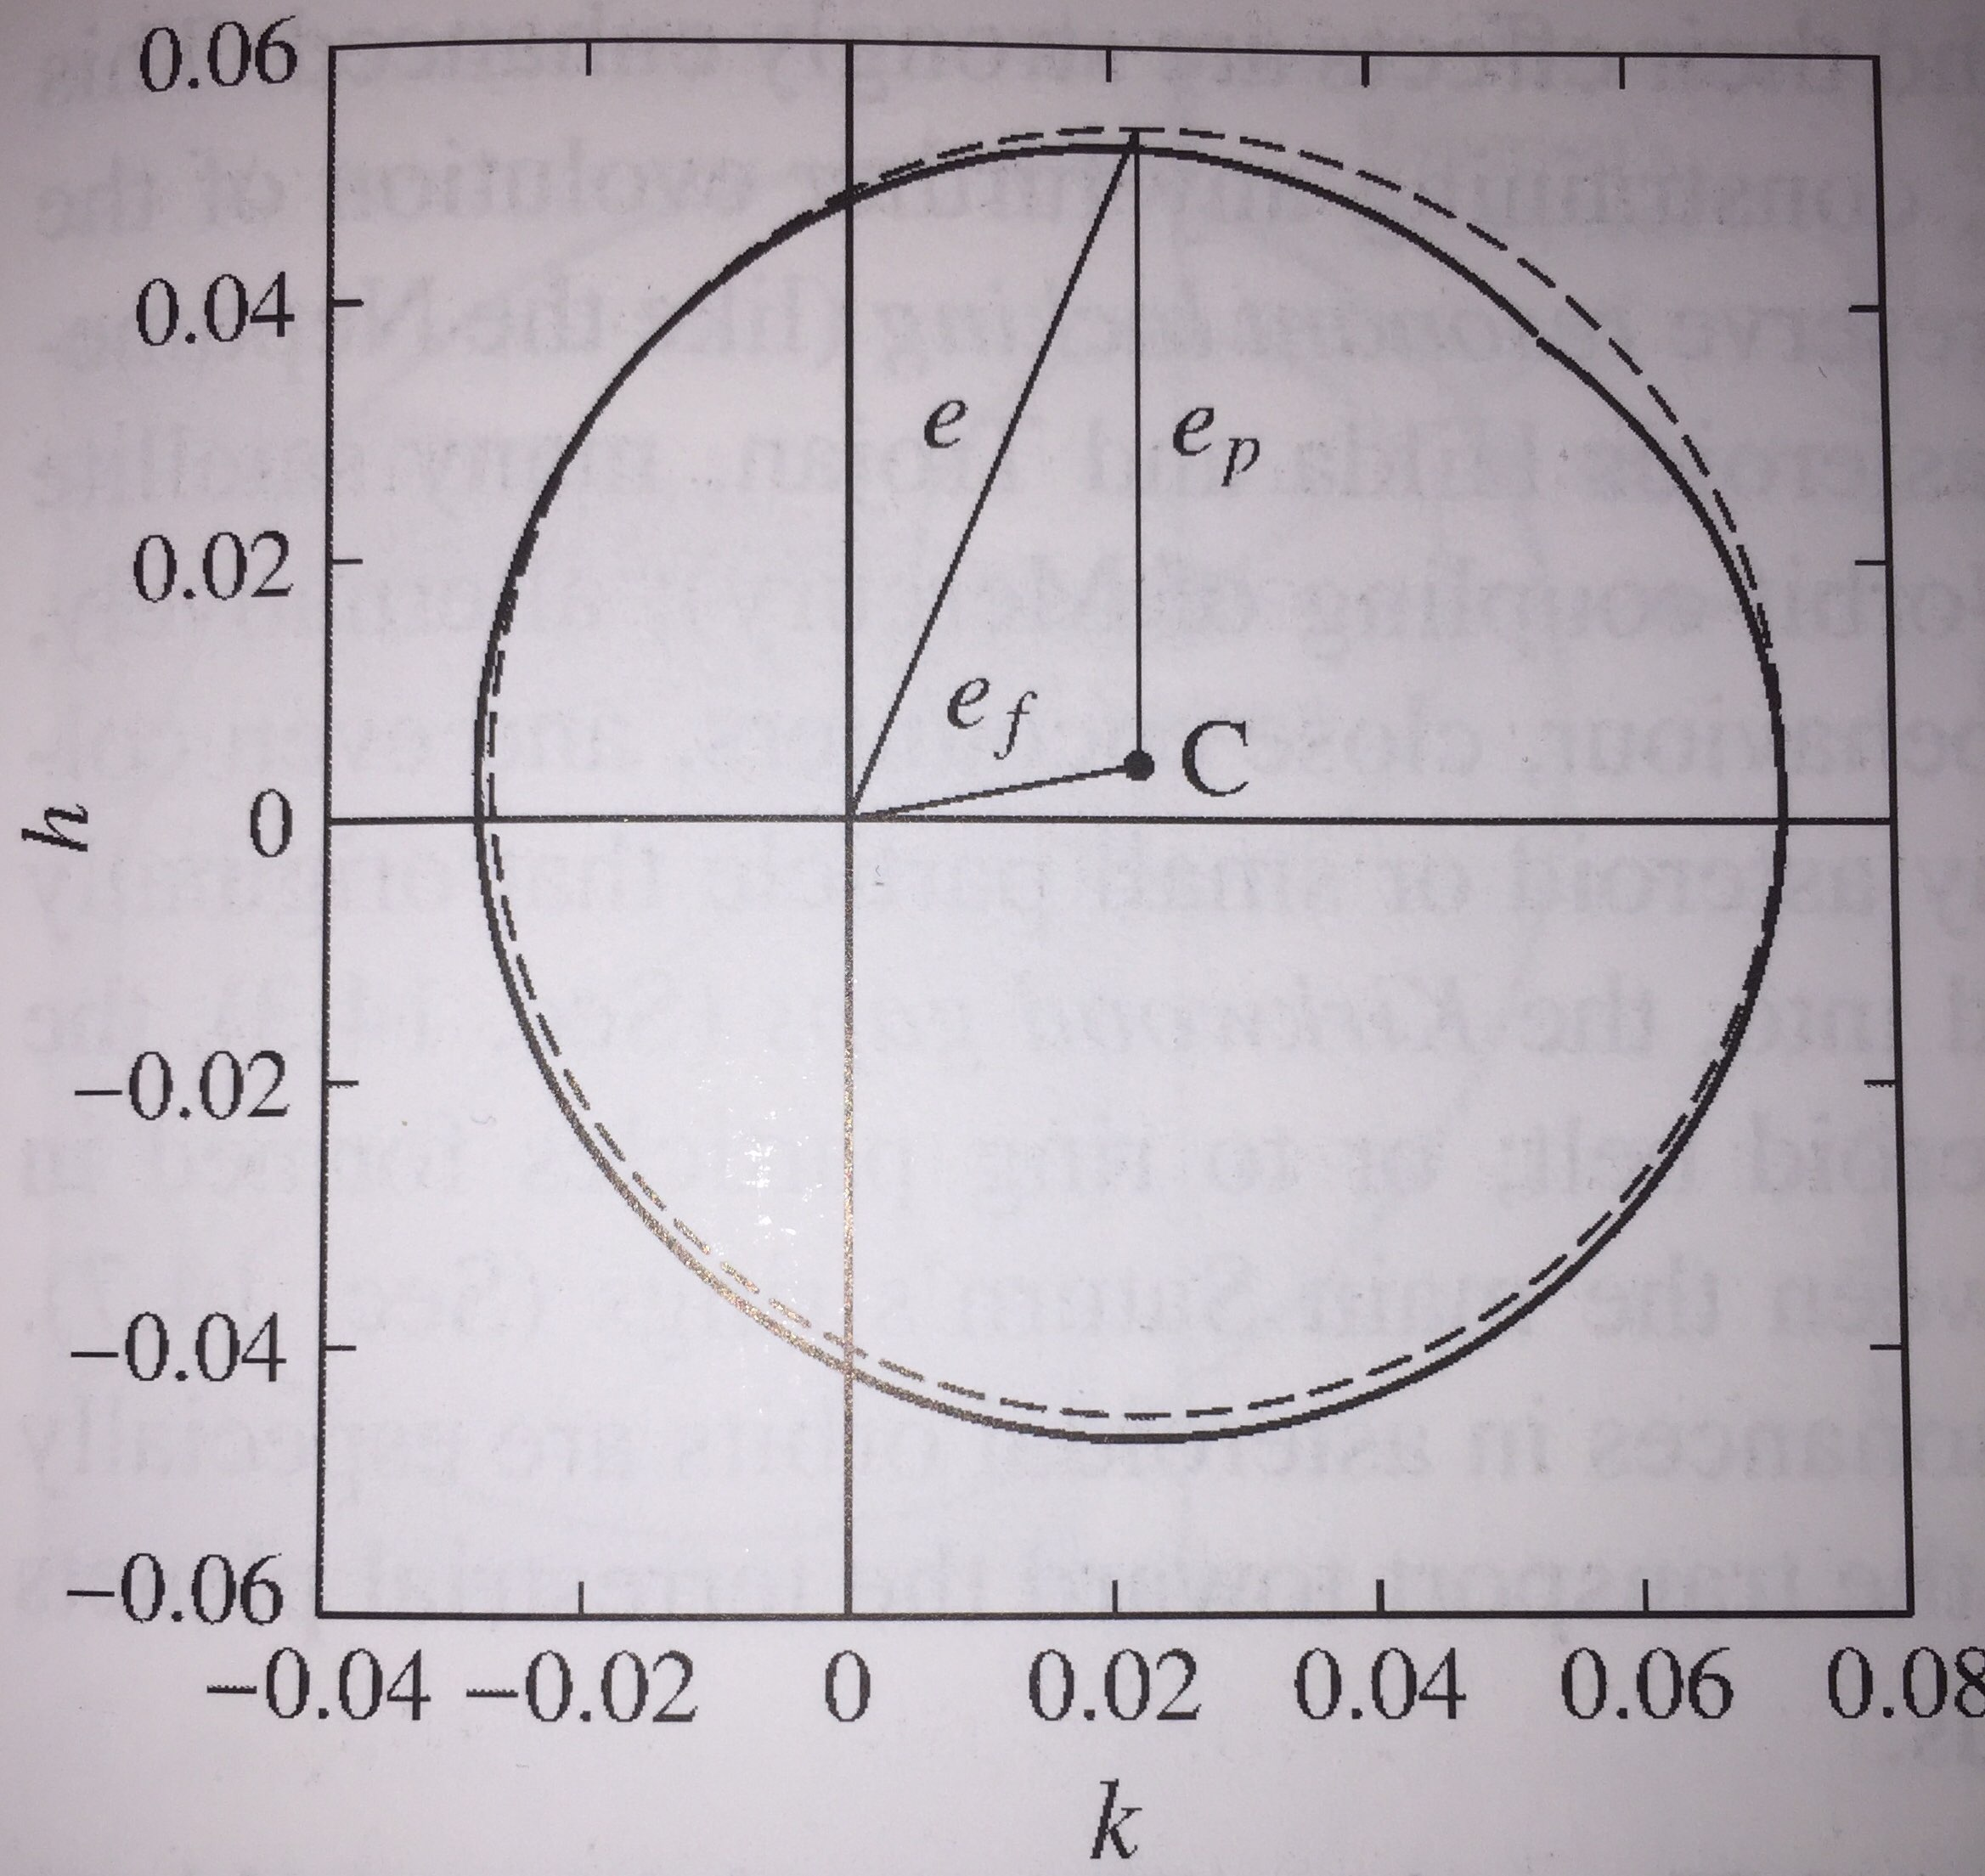
\includegraphics[keepaspectratio,width=0.7\textwidth]{forcedres}\end{figure}
\end{column}\end{columns}
\end{block}
\end{wordonframe}

\section{Resonances and chaotic evolution.}\linkdest{sec:resonanceschaos}

\begin{frame}{Resonances and ergodic behaviour}
\begin{columns}[T]
\begin{column}{0.45\textwidth}
\begin{figure}[!t]
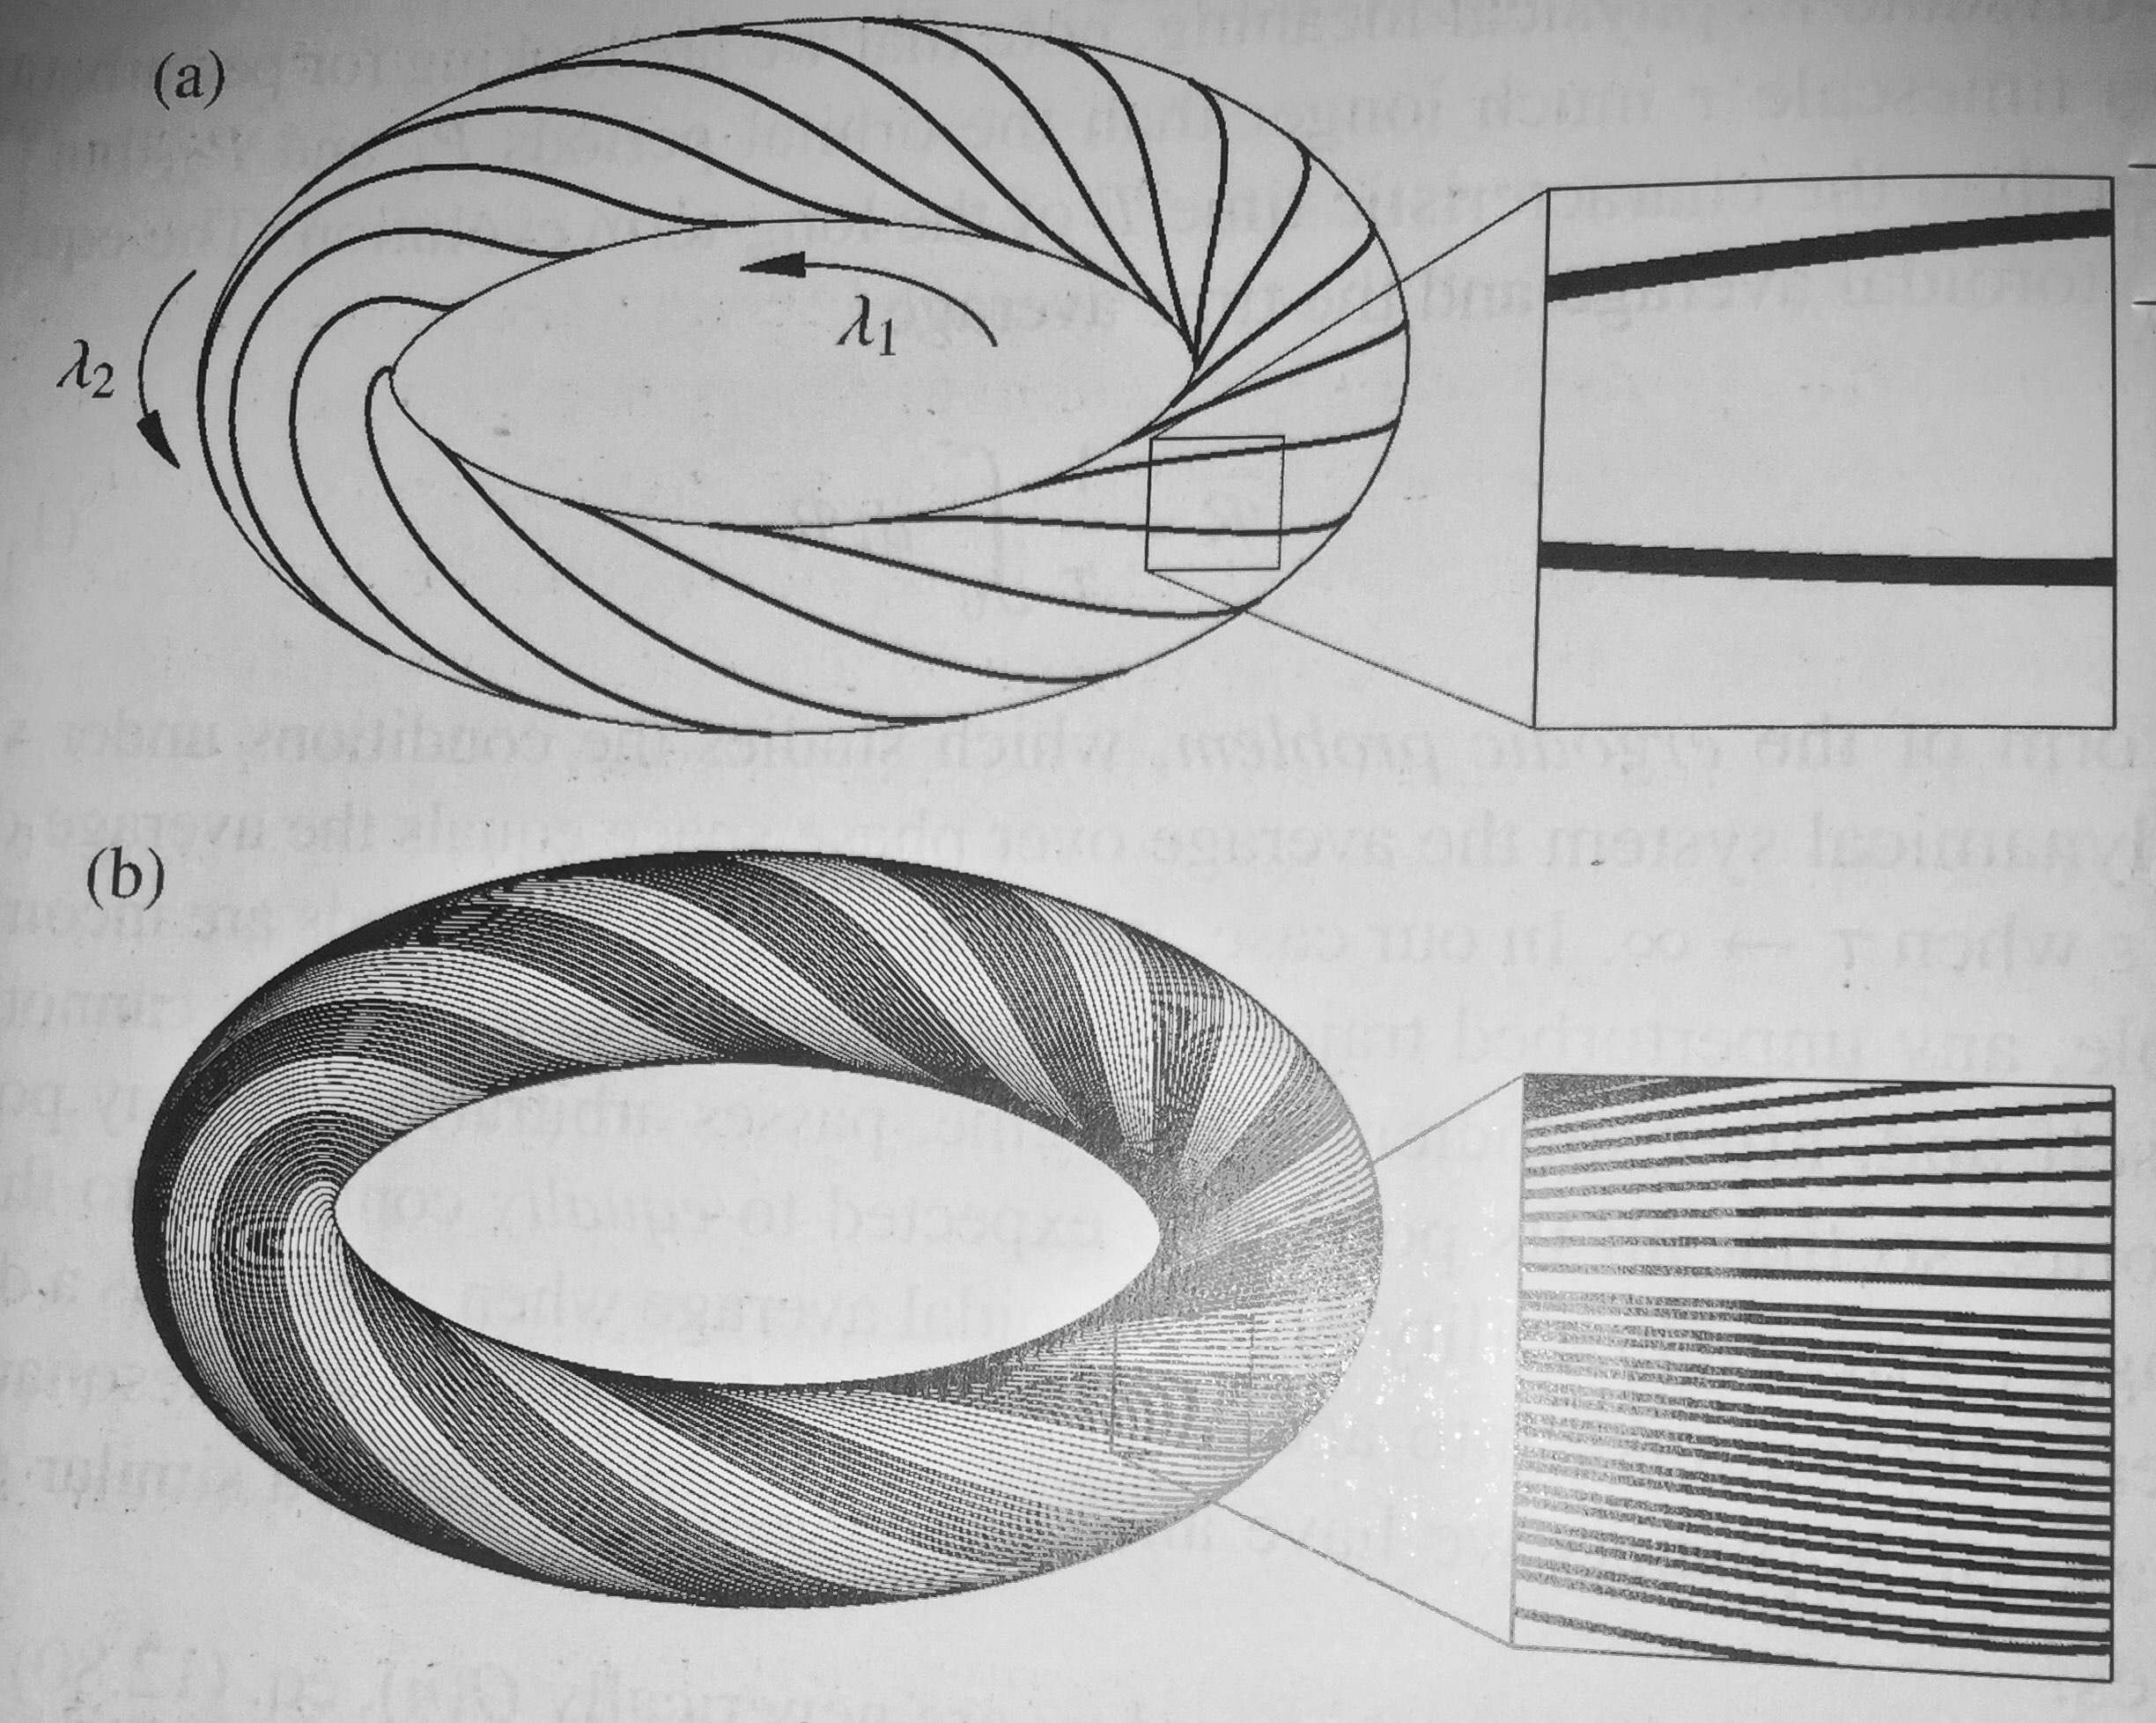
\includegraphics[width=0.9\textwidth]{resergo}
\end{figure}
Resonance condition (risonanze di moto medio): $i_1n_1+i_2n_2=0$.
secular effects (beyond lowest order in $\mu$):
\begin{align*}
&i_1(n_1+\dot{\epsilon}_1)+i_2(n_2+\dot{\epsilon}_2)+j_1\dot{\bar{\omega}}_1+j_2\dot{\bar{\omega}}_2\\
&+k_1\dot{\Omega}_1+k_2\dot{\Omega}_2=0
\end{align*}
\end{column}
\begin{column}{0.55\textwidth}
\begin{block}{Periodic pertutbation}
\begin{align*}
\bar{\phi_p}=\frac{1}{\tau}\int_0^{\tau}\phi_p\,d\tau
\end{align*}
elliptic orbit around oblate planet
\end{block}
\begin{block}{Non-periodic problem}
Two-planet system: average over torus $(\lambda_1,\lambda_2)$: $\exv{\phi_p}_{torus}$.
\end{block}
\end{column}
\end{columns}
\end{frame}

\begin{wordonframe}{Resonance and ergodicity}
\begin{block}{Torus in phase space: KAM theorem}
Figure: behaviour of $\phi_p$ for two body around primary (periodic) for resonant/non resonant case.
\begin{align*}
\exv{\phi_p}_{torus}=\frac{1}{(2\pi)^2}\int_0^{2\pi}d\lambda_1\,d\lambda_2\phi_p(\lambda_1,\lambda_2,\ldots)
\end{align*}
\end{block}
Ergodic problem: condition in dynamical system when average over phase space equal average over time to infinity.
A phase $\phi$ in $ C_{ijk}\cos{\Phi_{ijk}}$ is stationary: integrli del coseno crescono linearmente; non \'e valida ipotesi ergddica (equation for resonance including secular effects)
Secular resonance: $i_1=i_2=0$ ($\nu_6$ fascia asteroidale).
(Mimas and Tetis: tidal evolution have driven satellite from a multiplet line to another)
Risonanze: congelano stato dinamico o evoluzione caotica
\end{wordonframe}

\begin{frame}{Chaotic behaviour}
\begin{block}{Regime caotico}
Condizioni iniziali arbitrariamente vicine possono dar luogo a soluzioni molto diverse per grandi t.
Divisione spazio delle fasi in regione regolare e caotica.
\end{block}
\begin{block}{Esponente di Lyapunov}
The distance between two trajectories in phase space initially distant $\delta \gamma_0$ evolves $|\gamma(t)|=\delta\gamma_0\exp{\lambda t}$. $\lambda>0$ regime caotico (Lorenz 1963)

\end{block}
\end{frame}

\begin{wordonframe}{Comportamento caotico}
\begin{itemize}\item Mappa logistica: $x_{n+1}=Ax_n(1-x_n)$, per $A>3.57$ andamento caotico.
\item Ruota di Lorenz.
\begin{align*}
&\TDy{t}{m}=Q-km-\PDy{t}{m}\\
&m(\theta,t)=\sum_0^{\infty}[a_n(t)\sin{(n\theta)}+b_n(t)\cos{(n\theta)}]\\
&I\TDy{t}{\omega}=-\nu\omega+gr\int_0^{2\pi}m(\theta,t)\sin{\theta}\,d\theta=-\nu\omega+(\sum)\pi gra_n\\
&\TDy{t}{a_n}=n\omega b_n-Ka_n,\ \TDy{t}{b_n}=-n\omega a_n-Kb_n
\end{align*}
\end{itemize}
\end{wordonframe}


\section{Effetti dinamici della radiazione}\linkdest{sec:radiation}

\begin{frame}{Effetti della Radiazione}
\begin{columns}[T]\begin{column}{0.5\textwidth}
\begin{block}{Radiation/Gravity ratio}
$\beta=\frac{F_{rad}}{F_g}\propto\frac{S}{m}\approx\frac{\num{5.8e-5}}{\rho R}\approx\num{3e-10}$ ($R\approx\SI{1}{\kilo\meter}$, $\rho\approx\SI{1}{\gram\per\cubic\cm}$).
$G\msun{}\to(1-\beta)G\msun{}$.
\end{block}
\begin{block}{Variazione semiasse}
Equazione di Gauss: $\TDy{t}{a}=\frac{2T(a)}{n(a)}\propto a^{-2}a\expy{-\frac{3}{2}}\propto a\expy{-\frac{1}{2}}$.
\end{block}
\end{column} \begin{column}{0.5\textwidth}
\begin{block}{Effetto Poynting-Robertson}
Radiation force
\begin{equation*}
\vec{f}=Q_{pr}\frac{FS}{c}[(1-\hat{n}\cdot\frac{\vec{v}}{c})\vec{n}-\frac{\vec{v}}{c}]
\end{equation*}
Timescale of orbital circularization and decay: $\tau_d\approx\frac{mc^2}{FS}\approx\num{7e-6}(\frac{\rho}{\si{\gram\per\cubic\cm}})(\frac{R}{\si{\cm}})(\frac{r}{\si{\astronomicalunit}})^2\si{\year}$.
\end{block}
\end{column}  \end{columns}
\begin{block}{Effetto Yarkovsky}
Radiative recoil: l'effetto Y. \'e prodotto dal riscaldamento inomogeneo causato da una sorgente esterna.
$T_s=T_{eq}+\Delta T_s$. Infinite plane with periodic heat flux (toy model): $\Delta T_s\propto\exp{2\pi\nu t+\phi_t}$, temperature lags behind  flux.
Y recoil acceleration:
\begin{equation*}
\vec{f}_Y=-\frac{2}{3}\frac{\epsilon\sigma}{mc}\int_S\,dS\vec{n}_{\bot}T_s^4\approx-\frac{8}{3}\frac{\epsilon\sigma}{mc}T_{eq}^3\int_S\,dS\vec{n}_{\bot}\Delta T_s
\end{equation*}
\end{block}
\end{frame}

\begin{wordonframe}{Evoluzione dinamica: Effetti radiazione}
\begin{block}{Effetto Poynting-Robertson}
Radiation pressure: term $\propto\frac{1}{c}$.
$Q=Q_{ab}+gQ_{sc}$: g tiene conto dell'asimmetria tra forward/backward scattering.
\end{block}
\begin{block}{Effetto Yarkovsky}
Rotazione prograda/retrograda: accelerazione/decelerazione (a aumenta/diminuisce). Introduce rumore nella distribuzione nello spazio degli elementi orbitali delle famiglie dinamiche degli asteroidi.
\begin{equation*}
\tan{\phi_t}=-\frac{\Theta}{1+\Theta},\quad \Theta=\frac{\rho c_P\sqrt{\pi\chi\nu}}{4\epsilon\sigma T_{eq}^3}
\end{equation*}
Per corpèi inferiori al metro la conduzione riduce Yarkovsky.
Important for small NEO; a meteoroid (decine di metri): $\Delta a\approx 0.1\si{\astronomicalunit}$ (mean distance to Kirkwood gap) in few tens of \si{\mega\year}; a kilometer size asteroid: $\Delta a\approx 0.01\si{\astronomicalunit}$ (width of asteroid family) in \si{\giga\year}.
Eccesso NEO retrogadi: popolati da risonanze $\nu_6$ (bordo interno) e $3:1$ (intermedia) con uguale peso: dalla prima asteroidi che diminuiscono a.
\end{block}
\end{wordonframe}

\begin{frame}{Effetto YORP. Vento solare. Interazioni EM.}
\begin{block}{effetto YORP}\end{block}
\begin{columns}[T]\begin{column}{0.5\textwidth}
Oggetto di forma irregolare ($R<\SI{10}{\kilo\meter}$): trasferimento momento angolare (radiazione riflessa).
\end{column}
\begin{column}{0.5\textwidth}
\begin{align*}
&\TDy{t}{\omega}=\frac{\tau_z}{c}\\
&\TDy{t}{\theta}=\frac{\tau_{\theta}}{c\omega}\\
&\theta<(>)\deg{55}: \omega \uparrow(\downarrow)
\end{align*}
\end{column}  \end{columns}
\begin{block}{Solar wind}
Momentum flux $\propto\frac{1}{r^2}$: \num{3e-4} times smaller than radiation pressure. Drag ($\frac{v}{c}\to\frac{v}{v_w}$): $0.3$ times the Poynting-Robertson drag.
\end{block}
\begin{block}{EM interactions}
Ionization by UV, flux of electrons/ions. 
\end{block}
\end{frame}

\begin{wordonframe}{Effetto YORP. Vento solare. Interazioni EM. (e recap)}
\begin{block}{Effetto YORP}
\begin{align*}
d\vec{\tau}=\vec{r}\wedge\vec{f\,dA},\ \vec{f}=-\frac{2F_S\cos{\theta}\hat{n}}{3c}
\end{align*}
(Rubincam 2000). Rende gli assi ortogonali al piano orbitale.
\end{block}
\begin{block}{Solar wind}
$\rho_W\approx\SI{e-23}{\gram\per\cubic\cm}$, $v_W\approx\SI{400}{\kilo\meter\per\second}$.
\end{block}
Addensamento al bordo dello spazio degli elementi orbitali.
La dimensione dell'oggetto determina la velocit\'a di migrazione: stima et\'a delle famiglie.
\begin{block}{Solar wind}
For particles smaller than \SI{0.1}{\micro\meter} orbital decay is mainly due to solar wind drag.
\end{block}
\begin{block}{EM interactions}
A body in a plasma with $n_e$ charges negative until $\phi_e\approx KT/e$ restore equilibrium (extended over distance $\lambda_D$): for body smaller than \SI{1}{\micro\meter} is relevant Lorentz acceleration $qvB/(mc)\propto\frac{1}{R^2}$.
Planetary rings: particles motion is influenced by surrounding plasma and planet magnetic field. (Lorentz resonances: magnetic field frequency commensurable to particle's epicyclic frequencies).
\end{block}
\end{wordonframe}


\subsection{Evoluzione dinamica del sistema sistema solare. Stabilit\'a.}

\begin{frame}{Simulazioni}

\end{frame}
\begin{wordonframe}{simulazioni numeriche}

\end{wordonframe}
        
\section{Evoluzione collisionale}\linkdest{sec:collisions}

\subsection{Erosione, craterizzazione, rottura catastrofica}

\begin{frame}{Effetti degli urti}
\begin{columns}[T] \begin{column}{0.7\textwidth}
\begin{block}{Shattering/Dispersion: ri-accumulazione}
\begin{itemize}\item Energia d'impatto per unit\'a di massa del bersaglio perch\'e si abbia rottura catastrofica. \item Distribuzione iniziale dei frammenti (shattering) \item Composizione bersaglio e rotazione\end{itemize}
\begin{equation*}f_1=\frac{\text{m greater fragment}}{M_b}\end{equation*}
Strenght: Minimo sforzo per rottura.
\end{block}
\end{column}\begin{column}{0.3\textwidth}
\begin{block}{Velocit\'a relativa}\begin{itemize}\item Sistema solare interno: $\SI{10}{\kilo\meter\per\second}$\item Pianeti giganti/asteroidi/TNO: $\si{\kilo\meter\per\second}$\end{itemize}
\end{block}
\end{column}\end{columns}
\begin{itemize}\item Erosione \item Craterizzazione \item Rottura catastrofica
\end{itemize}
\end{frame}

\begin{wordonframe}{Effetti degli urti}
\begin{block}{Velocit\'a di fuga}
$v_e=\sqrt{\frac{2GM}{r}}=r\sqrt{\frac{8\pi G\rho}{3}}$, per $\rho\approx\SI{2}{\gram\per\cubic\cm}$: $v_e(\si{\meter\per\second})=r(\si{\kilo\meter})$
\end{block}
\begin{block}{Strenght}
Strenght: Minimo sforzo (Forza/superficie o energia/volume) per rottura (per compressione/tensione, impatto).
\end{block}
\begin{block}{Bersglio di basalto}
Basalto: $S\approx\SI{e7}{\erg\per\cubic\cm}$, $v_r=\SI{5}{\kilo\meter\per\second}$, $\frac{M_b}{M_p}\approx\num{e-4}$.
\end{block}
Fujiwara ('70): $f_1=0.5(\frac{SM}{\rho E/2})^{1.24}$.
Corpi soggetti a pressione hanno strength maggiore.
\end{wordonframe}

\begin{frame}{Distribuzione dei frammenti}
Collisioni a velocit\'a subsonica producono frammentazioni diverse
\begin{columns}[T]\begin{column}{0.5\textwidth}
\begin{block}{Massa}
$N(>m)\propto m\expy{-q},\ q\approx0.8$
\end{block}
\end{column}\begin{column}{0.5\textwidth}
\begin{block}{Velocit\'a}
$f(>v)\propto(\frac{v}{v_0})\expy{-k}$
\end{block}
\end{column}  \end{columns}
$F_{ke}=\frac{E_{ke}}{E_{imp}}$ cresce con energia specifica d'impatto secondo legge di potenza.
\end{frame}

\begin{frame}{Famiglie asteroidali}
\begin{block}{Limiti su S e $F_{ke}$ da osservazioni di asteroidi}
Asteroidi ($>\SI{150}{\meter}$) hanno $\tau_{spin}>\SI{2}{\hour}$: rubber piles (riaccumulazione: limite fissione, basso S,$F_{ke}$).
\end{block}
\begin{block}{Effetti delle collisioni su asteroidi ($R>\SI{100}{\kilo\meter}$)}
\begin{itemize}\item Famiglie dinamiche \item Asteroidi doppi \item LASPA: asteroidi di forma allungata (LA) e velocemente rotanti\end{itemize}
\end{block}
\end{frame}

\begin{wordonframe}{Risultanze di collisioni su asteroidi}
\begin{block}{LASPA: Ellissoidi triassiali di Jacobi.}
Urto che trasferisce grande momento angolare e frattura il corpo: $F_{ke}<\frac{2v_e}{v_i}$
\end{block}
\end{wordonframe}

\subsection{Deformazioni}

\begin{frame}{Deformazioni}
\begin{block}{Strain tensor}
\begin{align*}
&\epsilon_{ik}=\frac{1}{2}[\PDy{x_k}{\epsilon_i}+\PDy{x_i}{\epsilon_k}+(\PDy{x_i}{\epsilon_l}\PDy{x_k}{\epsilon_l})]:\ dV'=dV[1+\Tr{\epsilon}]
\end{align*}
\end{block}
\begin{block}{Stress tensor e equilibrio idrostatico}
\begin{columns}[T]\begin{column}{0.5\textwidth}
Forza per unit\'a di volume: $F_i=\PDy{x_k}{\sigma_{ik}}$.
\end{column} \begin{column}{0.5\textwidth}
Equilibrio idrostatico: $\PDy{x_k}{\sigma_{ik}}+\rho g_i=0$.
\end{column}  \end{columns}
Compressione uniforme: $\epsilon_{ik}=-\frac{P}{3K}\delta_{ik}$.
\end{block}
\begin{block}{Lavoro fatto a seguito delle deformazioni}
\begin{columns}[T]\begin{column}{0.5\textwidth}
\begin{align*}
&\int\delta W\,dV=\int\PDy{x_k}{\sigma_{ik}}\delta\epsilon_i\,dV\\
&\approx-\int\sigma_{ik}\delta\epsilon_{ik}\,dV
\end{align*}
\end{column}\begin{column}{0.5\textwidth}
\begin{align*}
&\sigma_{ik}=\Dcvar{\PDy{\epsilon_{ik}}{E}}{}=\Dcvar{\PDy{\epsilon_{ik}}{F}}{T}
\end{align*}
Materiale amorfo e isotropo:
$F=F_0+\mu(\epsilon_{ij}-\frac{1}{3}\delta_{ik}\epsilon_{ll})^2+\frac{K}{2}\epsilon_{ll}^2$
\end{column}\end{columns}
\end{block}
\end{frame}

\begin{wordonframe}{Strain, stress, thermodynamical quantities}
$[\sigma]=[S]=[P]=$Forza/superficie=Energia/Volume.
\begin{align*}
&dE=TdS+\sigma_{ik}\,d\epsilon_{ik}\\
&dF=-SdT+\sigma_{ik}\,d\epsilon_{ik}
\end{align*}
Piccole deformazioni: $F=F_0+\frac{\lambda_{iklm}}{2}\epsilon_{ik}\epsilon_{lm}$. In solido amorfo lo sviluppo in serie contiene scalari: $F=F_0+\frac{\lambda}{2}\epsilon_{ii}^2+\mu\epsilon_{ik}\epsilon_{ik}$.
K modulo compressione, $\mu$ deformazione di taglio ($\lambda$, $\mu$ coefficienti di Lam\'e).
$\Tr{\epsilon}=-\frac{P}{K}$.
\end{wordonframe}

\begin{frame}{Onde nei solidi}
\begin{columns}[T]\begin{column}{0.6\textwidth}
\begin{block}{Legge di Hooke}
\begin{equation*}
\sigma_{ik}=K\delta_{ik}\epsilon_{ll}+2\mu(\epsilon_{ik}-\frac{1}{3}\delta_{ik}\epsilon_{ll})
\end{equation*}
\end{block}
\begin{block}{Onde elastiche}
\begin{align*}
&\rho\ddvec{\epsilon}=[K+\frac{1}{3}\mu]\nabla(\scap{\nabla}{\epsilon})+\mu\nabla^2\vec{\epsilon}\\
&\PtwoDy{t}{\vec{\epsilon}_l}-c_l^2\nabla^2\vec{\epsilon}_l=0,\ c_l=\sqrt{\frac{K+4/3\mu}{\rho}}\\
&\PtwoDy{t}{\vec{\epsilon}_T}-c_T^2\nabla^2\vec{\epsilon}_T=0,\ c_T=\sqrt{\frac{\mu}{\rho}}
\end{align*}
\end{block}
\end{column} \begin{column}{0.4\textwidth}
\begin{block}{Onde longitudinali (unidirezionale)}
\begin{align*}
&\sigma_l=-\rho u_lc_l\\
&\sigma_T=\frac{\nu}{1-\nu}\sigma_l
\end{align*}
$\nu$ Poisson's ratio.
\end{block}
\end{column}  \end{columns}
\end{frame}

\begin{wordonframe}{Onde nei solidi}
\begin{align*}
&\epsilon_{ik}=\frac{1}{9K}\delta_{ik}\sigma_{ll}+\frac{1}{2\mu}(\sigma_{ik}-\frac{1}{3}\delta_{ik}\sigma_{ll})\\
&[K+\frac{1}{3}\mu]\nabla(\scap{\nabla}{\epsilon})+\mu\nabla^2\vec{\epsilon}=0
\end{align*}
\begin{columns}[T]\begin{column}{0.4\textwidth}\begin{block}{Intensit\'a}
\end{block}
\end{column} \begin{column}{0.6\textwidth}
\begin{block}{Stress onde longitudinali/trasversali}
\end{block}
\end{column}  \end{columns}
\end{wordonframe}

\begin{frame}{Hugoniot elastic limit}
\begin{columns}[T]\begin{column}{0.7\textwidth}
\begin{figure}[!ht]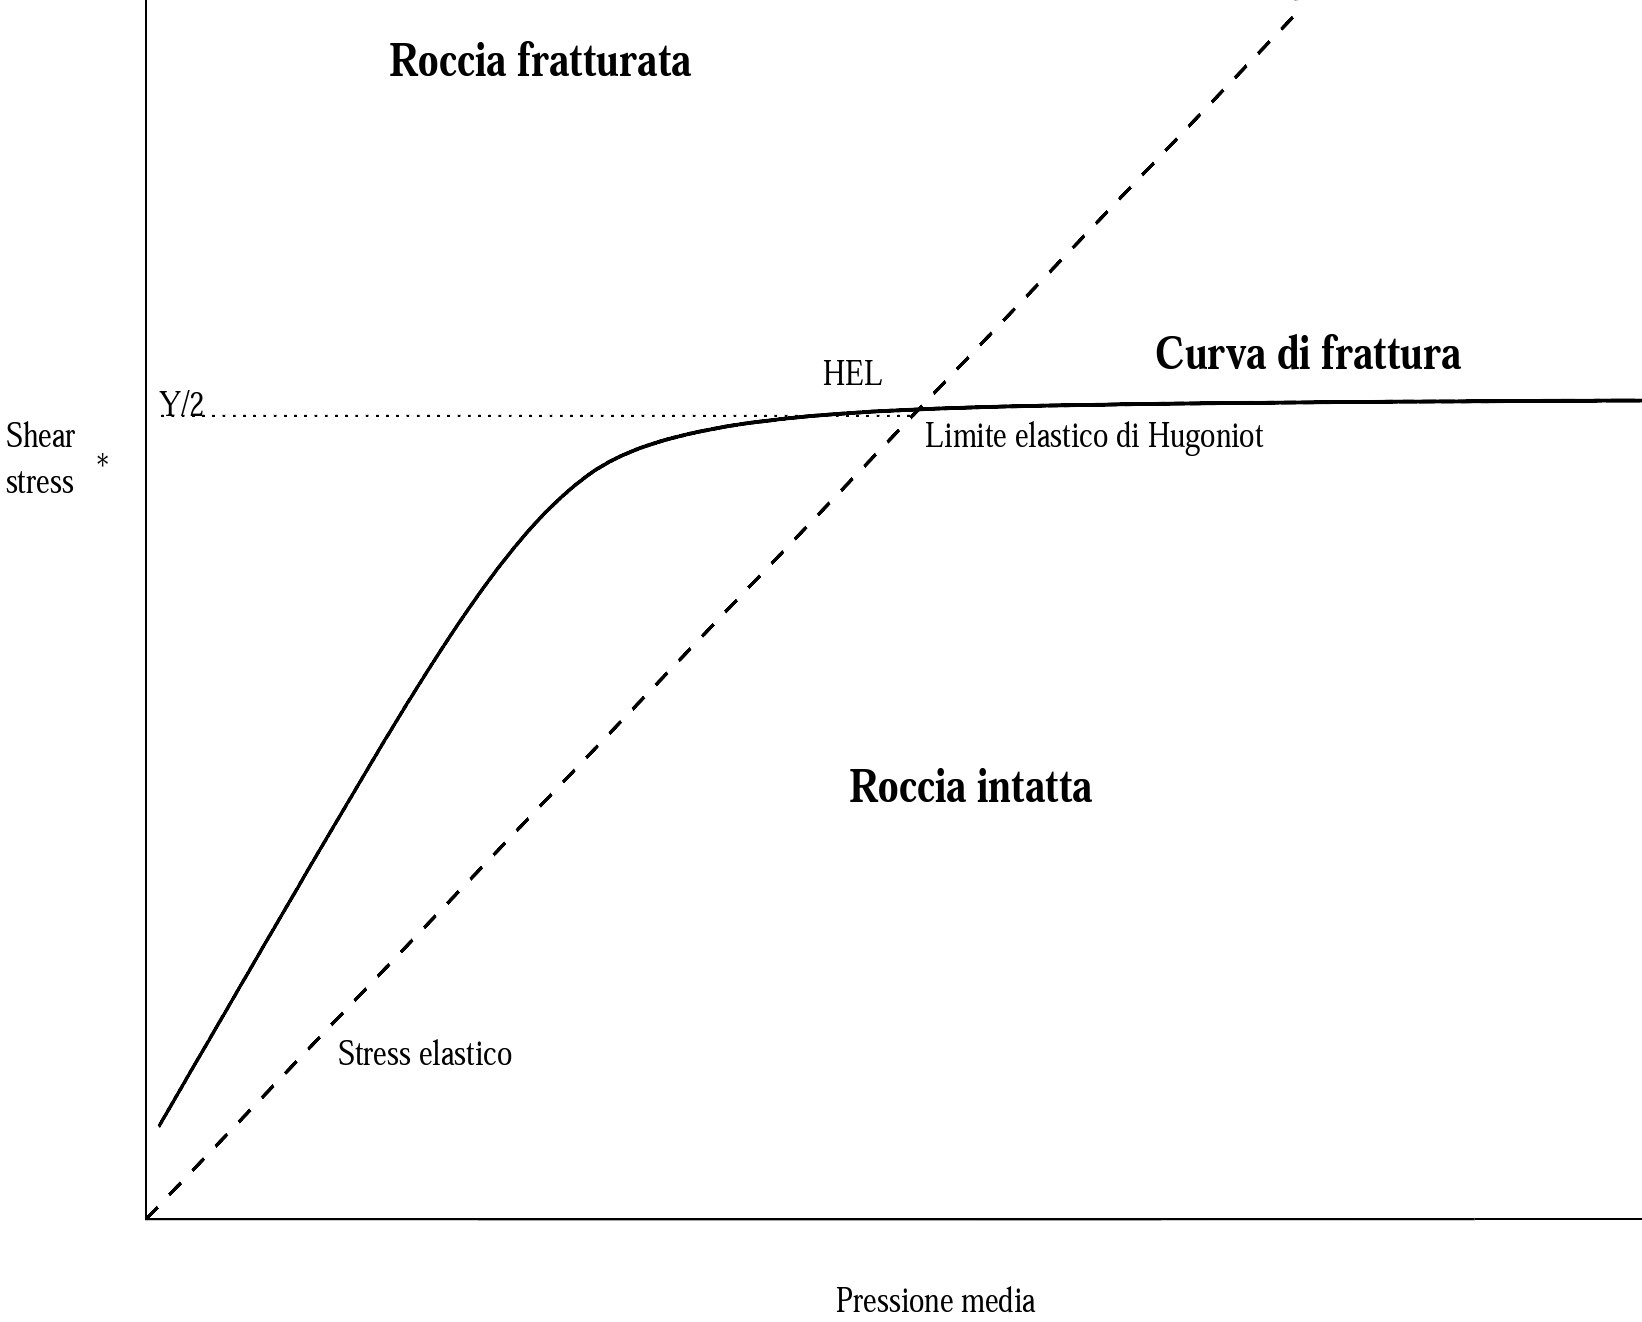
\includegraphics[keepaspectratio,width=0.9\textwidth]{shear}\end{figure}
\end{column} \begin{column}{0.3\textwidth}
\tikz\draw[->] (0,0) node[right] {Elastiche}--(0,1) node[right] {Onde d'Urto} node[midway,right] {Plastiche};
\begin{block}{Regime elastico}$|\sigma_l-\sigma_T|<Y$, Y yield stress.\end{block}
\end{column}  \end{columns}
\end{frame}

\begin{wordonframe}{HEL}
Suoerato il limite di Hugoniot si ha precursore elastico che si propaga con velocit\'a $c_l$ e onda plastica che si propaga con velocit\'a $c_b$: per $c_b>c_l$ si hanno onde d'urto.
\end{wordonframe}

\subsection{Teoria del danno}

\begin{frame}{Rottura}
\begin{block}{Distribuzione di Weibull}
Numero difetti attivi per deformazione $\epsilon$:
\begin{equation*}
N(\epsilon)=K\epsilon^m
\end{equation*}
$m$(materiale), $K\propto V$
\end{block}
Per rottura di corpi grandi in seguito a impatti ad alta velocit\'a siamo in regime di strength dinamica.
\begin{block}{Strain rate}
Vicino al punto d'impatto $\dot{\epsilon}\approx\frac{v_P}{l_P}$.
\end{block}
\end{frame}

\begin{wordonframe}{Teori del danno}
\begin{block}{difetti in seguito a urti}
Le onde dovute all'impatto attraversano il corpo e attivano processi di rottura; difetti crescono fino a dar vita a fratture macroscopiche.
\end{block}
\begin{block}{Transizione regime strength statica/dinamica}
Minima deformazione per rottura: $\epsilon_{min}\propto(K_0R^3)\expy{-\frac{1}{m}}$.
Strength tensile: $\propto\dot{\epsilon}\expy{\frac{3}{m+3}}\propto l_P\expy{-\frac{1}{4}}$.
\end{block}
\end{wordonframe}

\begin{frame}{Timing nei processi di urto}
\begin{itemize}
\item Allocazione energia d'impatto: estesa fratturazione
\item Espulsione frammenti a bassa velocit\'a: basso S basso $F_{ke}$. (Estesa fratturazione: strength/energy transfer bassa.)
\end{itemize}
\end{frame}

\begin{frame}{Modello di Grady-Kipp}
\begin{block}{Parametro di danneggiamento}
\begin{equation*}
\sigma_{ij}=K(1-D)\epsilon_{ll}\delta_{ij}+2\mu(1-D)(\epsilon_{ij}-\frac{1}{3}\epsilon_{ll}\delta_{ij})
\end{equation*}
\end{block}
\begin{block}{Fratture per unit\'a di volume $n$: $D=nV_f$}
\end{block}
\begin{block}{Evoluzione del danno nel tempo}
Le fratture crescono con velocit\'a $c_g$, $V_f=\frac{4}{3}\pi c_g^3t^3$:
\begin{equation*}D(t)=\int_{-\infty}^t\dot{n}(t')V(t-t')\,dt'=\frac{4}{3}\pi c_g^3\int_{-\infty}^t\TDy{\epsilon}{N}\dot{\epsilon}(1-D)(t-t')^3\end{equation*}
\end{block}
\begin{block}{Distribuzione dimensione frammenti}
\begin{equation*}
F(L)=\frac{\pi mK_0L^3}{12c_g}(t_f-\frac{L}{2c_g})\expy{m-1}\dot{\epsilon}^m
\end{equation*}
\end{block}
\end{frame}

\begin{wordonframe}{Grady-Kipp}
$t_f$ tempo a cui il danno \'e completo.
\end{wordonframe}



\end{document}